% %%%%%%%%%%%%%%%%%%%%%%%%%%%%%%%%%%%%%%%%%%%%%%%%%%%%%%%%%%%%%%%%%%%%%%%%%%%%%%%%
% %2345678901234567890123456789012345678901234567890123456789012345678901234567890
% %        1         2         3         4         5         6         7         8

% \documentclass[letterpaper, 10 pt, conference]{ieeeconf}  % Comment this line out if you need a4paper

% %\documentclass[a4paper, 10pt, conference]{ieeeconf}      % Use this line for a4 paper

% \IEEEoverridecommandlockouts                              % This command is only needed if 
%                                                           % you want to use the \thanks command

% \overrideIEEEmargins                                      % Needed to meet printer requirements.

% %In case you encounter the following error:
% %Error 1010 The PDF file may be corrupt (unable to open PDF file) OR
% %Error 1000 An error occurred while parsing a contents stream. Unable to analyze the PDF file.
% %This is a known problem with pdfLaTeX conversion filter. The file cannot be opened with acrobat reader
% %Please use one of the alternatives below to circumvent this error by uncommenting one or the other
% %\pdfobjcompresslevel=0
% %\pdfminorversion=4

% % See the \addtolength command later in the file to balance the column lengths
% % on the last page of the document

% % The following packages can be found on http:\\www.ctan.org
% %\usepackage{graphics} % for pdf, bitmapped graphics files
% %\usepackage{epsfig} % for postscript graphics files
% %\usepackage{mathptmx} % assumes new font selection scheme installed
% %\usepackage{times} % assumes new font selection scheme installed
% %\usepackage{amsmath} % assumes amsmath package installed
% %\usepackage{amssymb}  % assumes amsmath package installed

% % ----------------------------------------------------------------------------------------
% % Above content is from the RAS Latex template. 
% % ----------------------------------------------------------------------------------------

% % numbers option provides compact numerical references in the text. 
% % \usepackage[numbers]{natbib}
% \usepackage{multicol}
% \usepackage[bookmarks=true]{hyperref}

% %%%%%%%%%%%%%%%%%%%%%%%%%%%%%%%%%%%%wa
% % User commands.
% \usepackage{mathtools}
% \usepackage{amsfonts}  % for \mathbb
% \usepackage{graphics}
% \usepackage[pdftex]{graphicx}
% \usepackage{wrapfig}
% \usepackage{color}
% \usepackage{dsfont}
% % \usepackage[symbol]{footmisc}

% % % Algorithm.
% \usepackage{algorithmicx}
% \usepackage[ruled]{algorithm}
% \usepackage{algpseudocode}
% \usepackage{amssymb}

% % Caption
% \usepackage{caption}
% % \usepackage{subcaption}

% % Figure
% \usepackage{wrapfig}

% % ---------------------------------
% % User defined Macros
% % ---------------------------------

% \algnewcommand\algorithmicforeach{\textbf{for each}}
% \algdef{S}[FOR]{ForEach}[1]{\algorithmicforeach\ #1\ \algorithmicdo}

% % KL Divergence 
% \DeclarePairedDelimiterX{\infdivx}[2]{(}{)}{%
%   #1\;\delimsize\|\;#2%
% }
% \newcommand{\infdiv}{\infdivx}
% \newcommand{\kld}[2]{\ensuremath{D_{KL}\inf
% divx{#1}{#2}}}

% % Omit final dot from each def.
% \usepackage{expl3}
% \ExplSyntaxOn
% \newcommand\latinabbrev[1]{
%   \peek_meaning:NTF . {% Same as \@ifnextchar
%     #1\@}%
%   { \peek_catcode:NTF a {% Check whether next char has same catcode as \'a, i.e., is a letter
%       #1.\@ }%
%     {#1.\@}}}
% \ExplSyntaxOff
% \def\eg{\latinabbrev{e.g}}
% \def\etal{\latinabbrev{et al}}
% \def\etc{\latinabbrev{etc}}
% \def\ie{\latinabbrev{i.e}}

% % Vector.
% \let\vec\mathbf

% % Comments
% \providecommand{\kuan}[1]{{\color{blue} [Kuan: #1]}}
% \providecommand{\kuan}[1]{{\color{red} [Ashvin: #1]}}

% % ----------------------------------------------------------------------------------------
% % paper title
% \title{
% \LARGE \bf
% Planning to Practice: Efficient Online Fine-Tuning \\by Composing Goals in Latent Space
% }
% %%SL.2.23: This is a really nice title, though I wonder if this title only works if we have something like the reset-free system working? Without the reset-free, not quite clear if it's really "planning to practice" or just "planning to do the task"...
% %%AVN.2.21: I think "planning to practice" might be better for the reset-free story. Maybe something like "Scaffolding Online Fine-tuning of Long Horizon Tasks by Planning"?
% %%SL.12.28: I think it's a nice starting point for the title! I guess the idea you want to get across is that the planning component is what enables the learning to be autonomous, which makes a lot of sense. There are a number of unfortunate potential misunderstandings though that we should try to avoid:
% % 1. robotics people will tend to (mis)interpret "planning" as more traditional motion planning, which might make the title come across as kind of simplistic -- planning is a standard way to get autonomous robot behavior (and the autonomous *learning* part might be missed)
% % 2. some people might not quite get what the "autonomous learning" bit means, or that the paper has anything to do with RL at all
% % a few ideas for titles that kind of revolve around a similar theme but try to address some of these potential issues:
% % - Automating Real-World Goal-Conditioned RL via Goal Planning
% % - Planning with Goal-Conditioned Policies for Autonomous RL
% % - Autonomous Robotic Reinforcement Learning via Goal Planning

% \author{
% % Albert Author$^{1}$ and Bernard D. Researcher$^{2}$% <-this % stops a space
% % \thanks{*This work was not supported by any organization}% <-this % stops a space
% % \thanks{$^{1}$Albert Author is with Faculty of Electrical Engineering, Mathematics and Computer Science,
% %         University of Twente, 7500 AE Enschede, The Netherlands
% %         {\tt\small albert.author@papercept.net}}%
% % \thanks{$^{2}$Bernard D. Researcheris with the Department of Electrical Engineering, Wright State University,
% %         Dayton, OH 45435, USA
% %         {\tt\small b.d.researcher@ieee.org}}%
% Kuan Fang$^*$, Patrick Yin$^*$, Ashvin Nair, Sergey Levine\\
% University of California, Berkeley
% \thanks{$^{*}$Authors contributed equally to this work.}
% }

% \begin{document}

% \maketitle
% \thispagestyle{empty}
% \pagestyle{empty}

% \begin{abstract}
% % Training a robot to solve goal-reaching tasks can be expensive and time-consuming in complicated manipulation domains.
% %%AVN.2.21 I'm not sure about starting out with goal-reaching as the problem. In particular part of our novelty is realizing that goal-conditioning is a good solution to long horizon planning because you can be compositional. What do you think about the something like the following as motivation:
% %%SL.2.23: I agree with Ashvin here -- it's not obvious why goal reaching tasks are inherently desirable, and some justification like this would really help
% % Training a robot to solve long-horizon multi-step tasks can be expensive and time-consuming in complicated manipulation domains.
% % In the traditional reinforcement learning paradigm, such multi-step tasks are expensive to train as it does not take into account the temporal and semantic compositionality of the skills involved.
% % In this work, our key insight is that the combination of goal-conditioned RL, offline RL, and planning can allow agents to do so: temporal compositionality is achieved by planning over goals and semantic compositionality is achieved by the use of a goal-conditioned policy and contextual goal generator.
% % To address this problem, encouraging progress has been made in offline reinforcement learning using data previously collected in the same or related tasks.
% %%SL.2.23: At the level of the abstract, it's not quite clear to me what this is referring to or why offline RL is necessarily relevant (it becomes more obvious when reading the rest of the paper, but at this point in the writing, people might not get why you are talking about this)
% % However, effective pre-training and fine-tuning of a goal-conditioned policy to reach distant goals still remains an open question. In this work, we propose Planning to Practice (PTP), an approach that scaffolds online fine-tuning by exploiting the compositional structure of the offline data. Instead of directly commanding the policy to reach the desired final goal, our approach uses a planner to compose a sequence of subgoals to guide the policy during online fine-tuning. To propose diverse and feasible candidates for the planner, we train conditional subgoal generators on the offline data to recursively generate sequences of subgoals in the learned latent space. Using conditional subgoal generators of different temporal resolutions, we design a hierarchical planning algorithm that efficiently reduces the search space by finding subgoals in a coarse-to-fine manner. To further enhance the robustness of the planner, a latent plan buffer is devised to re-use previously selected plans as initial guesses in new episodes. We evaluate our method by pre-training on short-horizon demonstration data and fine-tuning to solve unseen multi-stage manipulation tasks in both simulation and the real world. Compared with existing methods, our approach produces plans of better quality and significantly improves the efficiency of the online fine-tuning of the goal-conditioned policy. 
% %%AVN.2.21 The abstract might be a little too detailed/go too low-level too soon
% %%SL.2.23: One of the things that seems non-ideal about the current abstract is that it doesn't quite communicate what the exciting new idea is. Perhaps a good narrative structure might look something like this: (1) explain why goal reaching stuff is good; (2) explain why hierarchical approach is desirable; (3) explain how online finetuning fits. It seems like the general gist of the method amounts to showing that hierarchy + finetuning makes goal-conditioned RL work. So maybe we can phrase the abstract kind of like this:


% % Reinforcement learning provides a promising approach for autonomously acquiring individual manipulation skills.
% % However, general-purpose robots in real-world settings might require large repertoires of behaviors.
% % In this case, an appealing proposition is to train multi-task policies that can perform a wide range of different behaviors on command.
% % Goal-conditioned reinforcement learning addresses this problem by training policies that reach a configurable goal, but such policies are notoriously difficult and time consuming to train.

% % Our experimental evaluation shows that we can learn temporally extended skills in the real-world after 60 minutes of finetuning.
% % (e.g., taking out an object from a drawer and then closing the drawer).

% General-purpose robots require diverse repertoires of behaviors to complete challenging tasks in real-world unstructured environments. To address this issue, goal-conditioned reinforcement learning aims to acquire policies that can reach configurable goals for a wide range of tasks on command. However, such goal-conditioned policies are notoriously difficult and time-consuming to train from scratch. In this paper, we propose Planning to Practice (PTP), a method that makes it practical to train goal-conditioned policies for long-horizon tasks that require multiple distinct types of interactions to solve. Our approach is based on two key ideas. First, we decompose the goal-reaching problem hierarchically, with a high-level planner that sets intermediate subgoals using conditional subgoal generators in the latent space for a low-level model-free policy. Second, we propose a hybrid approach which first pre-trains both the conditional subgoal generator and the policy on previously collected data through offline reinforcement learning, and then fine-tunes the policy via online exploration. This fine-tuning process is itself facilitated by the planned subgoals, which breaks down the original target task into short-horizon goal-reaching tasks that are significantly easier to learn. We conduct experiments in both the simulation and real world, in which the policy is pre-trained on demonstrations of short primitive behaviors and fine-tuned for temporally extended tasks that are unseen in the offline data. Our experimental results show that PTP can generate feasible sequences of subgoals that enable the policy to efficiently solve the target tasks.  
% \footnote{Supplementary video: \href{https://sites.google.com/view/planning-to-practice}{sites.google.com/view/planning-to-practice}}

% \end{abstract}

\section{Introduction}

% %% What is the problem?
% Utilizing large datasets for robotics -> GCRL from offline data
Developing controllers that can solve a range of tasks and generalize broadly in real-world settings is a long-standing challenge in robotics.
Such generalization in other domains such as computer vision and natural language processing has been attributed to training large machine learning models on massive datasets~\citep{krizhevsky2012imagenet}.
Consequently, one promising approach to robustly handle a wide variety of potential situations that a robot might encounter is to train on a large dataset of robot behaviors.
Prior work in robotics has demonstrated effectively generalization from training on large datasets for individual tasks, such as grasping~\citep{levine2017grasping, yu2021conservative}.
%%SL.3.1: It would be good to cite more non-conflicted papers, such as Lerrel's grasping paper, the Dieter Fox IRIS paper, and as many other relevant non-conflicted papers as you can find.
However, a general-purpose robot should be able to perform a wide range of skills, and should also be \textit{taskable}.
That is, it must be able to complete a specific task when specified by a human, including temporally extended tasks that require sequencing many skills together to complete.
This topic has been studied in prior work on goal-conditioned reinforcement learning, where a robot aims to perform a task given a desired end state~\citep{Khazatsky2021WhatCI, chebotar2021actionable, kalashnikov2021mtopt}.
%%SL.3.1: My suggestion: add many more citations, and also add "or other type of command~\citep{}" and add a bunch more citations. Don't skimp on citations, and definitely make sure to cite plenty of non-conflicted papers.
What remains to make these methods widely applicable for real-world robotics?
%%SL.3.1: It's good to pose questions, but it's not good to pose very open-ended questions, because this encourages lateral thinking (i.e., the reader will try to answer the question, and possibly not in the way that you expect). Perhaps a better organization would be to delete the above sentence and move the beginning of the next para (which explains the issues with GCRL) into the above para, and then start the next para by talking about the solution?
% Can the same approach, which has the benefit of requiring little human supervision, also be used to learn temporally extended tasks?

% % What is the problem? Long-horizon self-supervised RL OR Scaffolding long horizon policies
% % Scaffolding long horizon policies
% % Insight: (initial-state conditional) goal-conditioning allows you to compose subskills via planning
% % Insight: finetuning is required because 1. offline RL may not be perfect 2. there are errors from stitching skills together that must be corrected
% % Insight: planning can be a scaffold, but finetuning lets you train long-horizon goal-conditioned policies when you have the data
% % Online finetuning of long horizon policies via goal-conditioned planning
% A general purpose robot that is useful in unstructured environments must be able to perform a vast array of skills, and be \textit{taskable}.
% That is, it must be able to complete a specific task when specified by a human, including temporally extended tasks that require sequencing many skills together to complete.
% Deep reinforcement learning (RL) is a promising approach towards learning individual skills by optimizing a policy to maximize expected returns provided a reward function, and significant progress has been made on improving policy optimization.
% %%KF.2.26 Maybe it would be better to add 1-2 sentences to explain why GCRL is good for learning diverse tasks. I can think of several points, but Ashvin can probably summarize better:
% % - Configurable: Easy to specify tasks and rewards.
% % - Versatility: Can better share knowledge across different tasks of arbitrary horizons and efficiently reuse collected experiences.
% % - Compositionality: Goals can naturally serve as plans or curriculum in GCRL. 
% However, questions remain on how to apply deep RL in practice to train generalist robots that can accomplish useful tasks.
% One solution is self-supervised goal-conditioned RL, which learns general-purpose policies that aim to reach user-specified goal state.
% %%KF.2.26 The end of the first paragraph and the beginning of the 2nd paragraph are a bit disjointed. Maybe we could move the following sentences to the beginning of the 3rd paragraph instead.
% %%AVN.2.26 I see what you mean, we could potentially talk about how long horizon is a general case of GCRL here - I think we have to decide which flow to go with
% Prior work has showed how goal-conditioned RL utilizing prior data can learn taskable skills specified by a goal image without an external reward function~\citep{Khazatsky2021WhatCI}.
% %%SL.2.27: Maybe above sentence can be rephrased a bit more broadly, along the lines of something like: Prior work has studied varies methods for training goal-conditioned policies~\citepp{lots_of_citations}, including [whatever]. [basically, include more than just one conflicted citation to acknowledge there is tons of research on this]
% This is accomplished by learning an affordance model on the offline trajectories that predicts potential goals in a scene, and offline RL to learn a policy from the same offline data.
% %%SL.2.27: The whole "affordance model" part is kind of coming out nowhere (not clear why it's important, necessary, or what it has to do with the preceding motivation)
% Can the same approach, which has the benefit of requiring little human supervision, be used to learn temporally extended tasks?
% % How can we learn to compose a set of skills from prior data?
% %%SL.2.27: Something in this logical chain feels missing -- I think it's the jump from "goal conditioned RL" to "temporally extended tasks". Perhaps another sentence is needed to "fill in the blank" about why temporally extended tasks are important? Basically something that just states but we really want temporally extended tasks, and these are hard (maybe the next para says this, but then the above sentence feels premature)

\begin{figure}[t!]
    \centering
    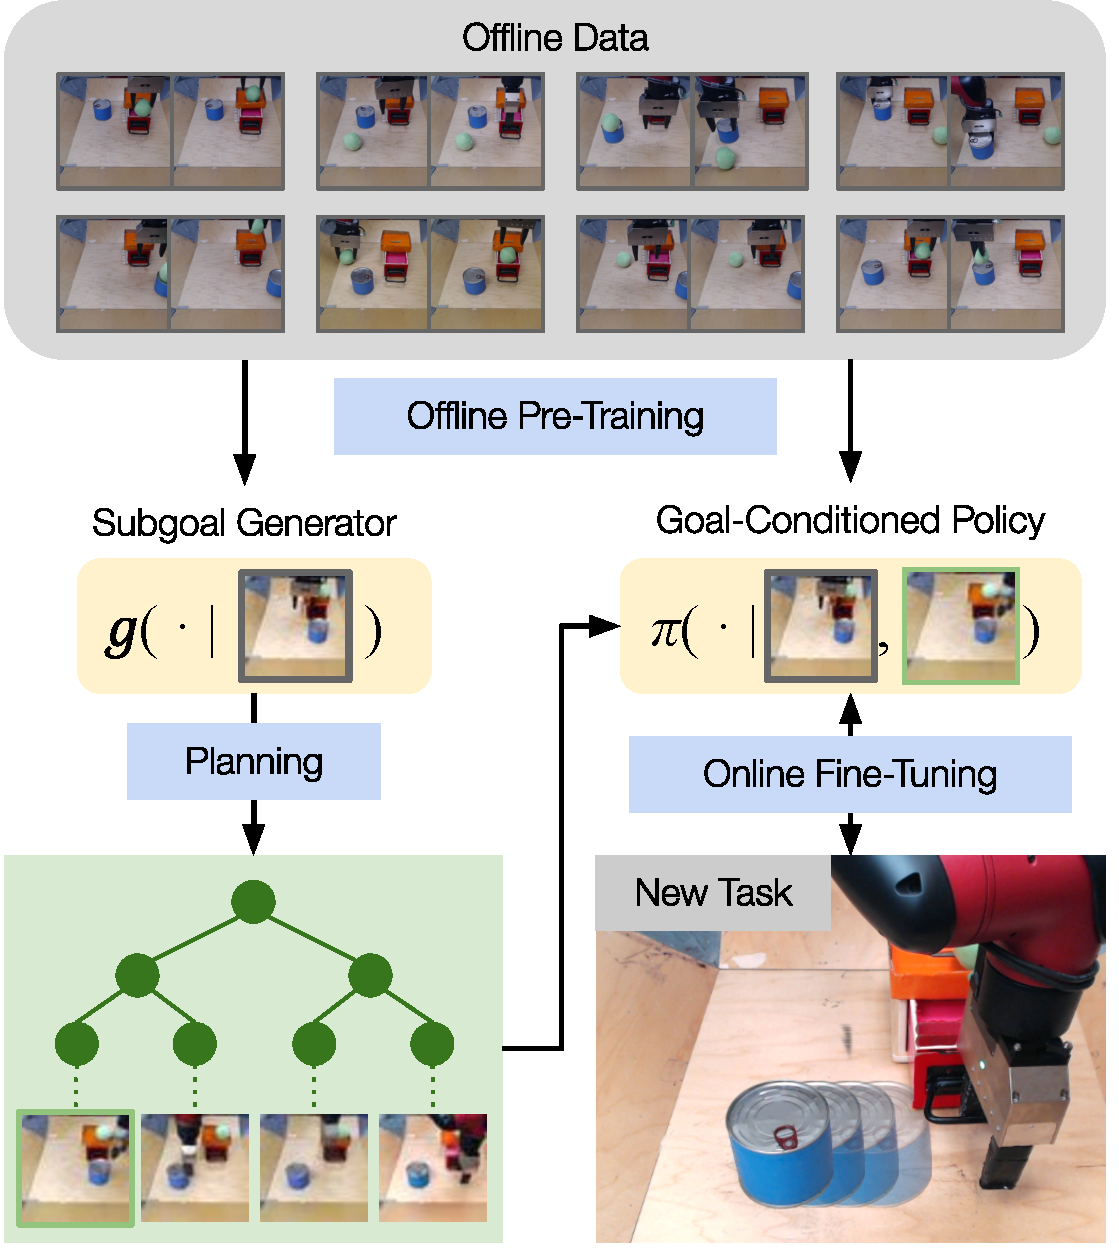
\includegraphics[width=.6\textwidth]{ptp/figures/intro.pdf}
    % \includegraphics[width=.4\textwidth]{example-image-a}
    % \vspace{-6mm}
    \caption{Our method, Plan to Practice (PTP), solves long-horizon goal-conditioned tasks by combining planning and fine-tuning.
    %%SL.3.1: See my comments before about planning having (usually) a pretty different meaning in robotics... without context, this is likely to lead to a misunderstanding.
    We begin with an offline dataset containing a variety of behaviors, and train a subgoal generator and goal-conditioned policy on this data. Then, to learn a more complex multi-stage tasks, we optimize over subgoals using the subgoal generator, which corresponds to a planning procedure over (visual) subgoals, and fine-tune the policy with online RL by practicing these subgoals. This enables the robot to solve multi-stage tasks directly from images.}
    %%SL.3.1: I edited the caption a fair bit. Generally, be careful not to inadvertently overclaim (variety of environments, new tasks, etc.). Readers will see right through it, and your credibility will be shot. Then they won't believe anything you say.
    \label{fig:intro}
    %\vspace{-5mm}
\end{figure}

While goal-conditioned policies can be trained effectively for relatively short-horizon tasks, temporally extended multi-stage can pose a significant challenge for current methods. These tasks present a major exploration challenge during online learning, and a major challenge for credit assignment during offline learning.
%%SL.3.1: I edited the sentences below and replaced them with the one above. I edited the paragraphs below to better address exploration, but the "credit assignment" bit is a bit artificial, maybe there is a clearer term we can use that would fit with the next two paragraphs better? not sure...
%One challenge is in solving long-horizon, temporally extended tasks.
% Why is it interesting and important
%Goal-conditioned RL in theory can represent long horizon tasks as simply another task to generalize to.
%In practice, reinforcement learning with long-horizon tasks is known to be a difficult problem due to the challenges of exploration and credit assignment across a long time horizon.
%But unique challenges and opportunities appear in the context of goal-conditioned RL.
%%KF.2.26 Should we also talk about the challenges in terms of exploration and credit assignment across a long time horizon?
%%AVN yes, added above
%%SL.2.27: I'm actually confused by the above motivation: it says long-horizon is hard, but self-supervised (why?) goal-conditioned RL solves it. That feels like a non-sequitur -- we were saying before we want goal-conditioned, so if it just solves it, why do we need this paper? And in what sense is it self-supervised? Perhaps it would be cleaner to simply say that we want long-horizon goal-conditioned stuff [because of some reason], and this is hard, because while long-horizon RL is hard already, goal-conditioned long-horizon RL is even harder [with citations]
% While long-horizon tasks are in general more difficult, goal-conditioning offers the chance for composition.
% Training a long horizon policy without considering the sequencing of tasks
%%SL.2.27: what does that mean?
% may require an amount of data that is exponential in the length of the sequence.
%%SL.2.27: any RL problem may require an exponential amount of data, so this statement is largely meaningless
In this chapter, we aim to address these challenges by combining two ideas. The first is that long-horizon goal-reaching tasks can be decomposed into shorter-horizon tasks consisting of subgoals. The second is that these subgoals can be used to \emph{fine-tune} a goal-conditioned policy online, even if its performance from offline data is poor.
% If we could compose skills together autonomously by sequentially setting coherent subgoals, the .
%%SL.2.27: Talking about sample efficiency here seems like a red herring, the issue is not just sample efficiency but being able to train policies that work at all.
% One idea that can be used to compose skills is conditional generative models of goals.
% Affordance models provide exactly this kind of knowledge: potential subgoals that can be reached from a given observation.
%%SL.2.27: reader doesn't know what an affordance model is at this point
The first idea enables us to address the exploration challenge, by automatically generating intermediate subgoals that can be ``practiced'' on the way to a longer-horizon final goal. In the framework of goal-conditioned RL, solving long-horizon tasks can be reduced to the problem of optimization over a sequence of subgoals for the goal-conditioned policy, and this optimization over subgoals can be regarded as a kind of high-level planning, where the optimizer selects waypoints for achieving a distant goal. The high-level planner itself can use a learned high-level model.

% This suggests that the key missing element is planning: by planning over future sequences, an agent can compose these kills.
% The plans can be provided to the lower level policy.
%%SL.2.27: As far as I can tell, the main idea in this paragraph is that the challenges of training long-horizon goal-conditioned policies can be overcome with [something]. But the [something] is not really explained (just the label "affordance model" is used without explanation). Perhaps it would be good to clearly and explicitly state the point (long-horizon + goal is hard, we can chain goals to make it easier), and try to more clearly define what "affordance" means (or use another more self-explanatory term)

%%KF.2.26 It might be better to motivate the utilization of offline data before talking about online fine-tuning?
%%AVN.2.26 I kind of quickly introduced offline data along with VAL above but maybe we need to expand on it more
However, if we rely entirely on offline data, credit assignment challenges make it difficult to perform longer-horizon tasks even with subgoal planning. Even if the offline RL policy performs well on each individual skill, there may be errors from stitching skills together because the initial states of each stage diverge from the offline data when they are composed together. In practice, this leads to poor performance when using only offline training. Therefore, the second key idea in our work is to utilize subgoal planning not merely to \emph{perform} a multi-stage task, but also to make it possible to \emph{practice} that task to finetune it online. While online training for temporally extended tasks is ordinarily difficult, by addressing the exploration challenge with subgoal planning, we make it possible for the robot to practice a series of relatively short-horizon tasks, which makes this kind of finetuning feasible. Thus, the planner acts both as a higher level policy when performing the task, and as a scaffolding curriculum for finetuning the lower-level goal-conditioned policy
%%SL.3.1: Rewrote the material below
%Composing subgoals in this manner from offline data, however, runs into the issue of distribution shift.
% With this kind of hierarchical approach, 
% there may be two issues.
%Especially if there are differences between the offline data and test environment, offline RL may not be perfect.
%%SL.2.27: Major disconnect here -- neither "hierarchical" nor "offline RL" were introduced before
%Even if the offline RL policy performs well on each individual skill, there may be errors from stitching skills together because the initial states of each stage diverge from the offline data when they are composed together.
%One solution to these problems of distribution shift is online fine-tuning.
By collecting data actively in a specific environment, we can directly experience the distribution shift and can use reinforcement learning to improve performance under this shift.
%Additionally, since the data that is collected is entire trajectories, this data can be used to fine-tune the long horizon goal-conditioned policy to actually solve the task directly.
%In this way, the planner can either act as a higher level policy to solve the task, or simply a scaffolding curriculum for the lower level goal-conditioned policy until the goal-conditioned policy can solve specific long-horizon tasks itself.
%%SL.2.27: Generally, I think this paragraph plays an important role: it serves to introduce the (highly nontrivial) idea that goal-conditioned + stitching multiple goals together by optimizing subgoals ("planning") can work very well if combined with offline RL and online finetuning. This is a subtle and extremely important idea. Right now the explanation though is pretty messy, maybe consider rewriting this paragraph, and make sure that any new concept (like offline RL) is introduced and there is a clear logical progression from the previous paragraph.

% Your approach
% Our technical contributions
To this end, we propose Planning to Practice (PTP), an approach that efficiently trains a goal-conditioned policy to solve
%%SL.2.24: It might be non-obvious in what sense the tasks are novel (and are they novel? if not, then maybe omit this part)
%%AVN.3.1 Took out "novel"
multi-step tasks by setting subgoals to exploit the compositional structure of the offline data.
%%SL.2.24: Hmm... so this presents the key idea as "exploiting the compositional structure of the offline data" -- is that really the key idea?
%%SL.2.27: same comment... not clear how the structure of the offline data is coming in; do you just mean that this is where affordances come from?
An outline is shown in Fig.~\ref{fig:intro}. Our approach is based around a planner that composes generated subgoals
% in the learned latent space
%%SL.2.27: what latent space?
%%AVN.3.1 we don't talk about latent spaces so far and its not that vital to the story so I'll just take it out
to guide the goal-conditioned policy during an online fine-tuning phase.
To propose diverse and reachable subgoals to form the candidate plans, we design a conditional subgoal generator based on conditional variational autoencoder (CVAE)~\citep{sohn2015cvae}.
Through training on the offline dataset, the conditional subgoal generator captures the distribution of reachable subgoals from a given state and generates sequences of subgoals from the learned latent space in a recursive manner.
%To efficiently find a feasible sequence of subgoals that leads to the desired goal state, we propose an efficient sampling-based planning algorithm using the conditional subgoal generator.
%%SL.3.1: commented out above sentence (it seems kind of uninformative at this level of detail, given that the reader won't have much context)
Our subgoal planning algorithm hierarchically searches for subgoals in a coarse-to-fine manner using multiple conditional subgoal generators that trained to generate goals at different temporal resolutions.
%We further devise a latent plan buffer that re-uses the previously selected plans as initial guesses in new episodes to enhance the chance of finding the plan.
%%SL.3.1: commented out the above (too low level, makes the method kind of come across as a bag of hacks)
Both the goal-conditioned policy and the conditional subgoal generators are pre-trained on the offline data, and the policy is fine-tuned on the novel target task. 
%%SL.2.24: Generally, this paragraph is reasonable, but a bit disorganized. I would recommend trying to structure it more top down, starting with the key ideas and subordinating the design choices under those key ideas.

% Summary of contributions
% Our experimental results.
%%SL.2.24: Maybe it would be better to have the first half of this paragraph clearly state the contributions of the work. This is especially important since it might not be entirely obvious to some readers what *precisely* is novel in the paper, so starting with a few sentences to explain the main contribution would remove this issue. If we can't clearly state the novel contribution in a few sentences here, it's likely the reviewers won't understand what the key contribution is either.
Our main contribution is a system for learning to solve long-horizon goal-reaching tasks by fine-tuning the goal-conditioned policy with subgoal planning in a learned latent space. 
We evaluate our approach on multi-stage robotic manipulation tasks with raw image observations and image goals in both simulation and the real world.
After being pre-trained on short demonstrations of primitive interactions, our approach is able to find feasible subgoal sequences as plans for unseen final goals by recursively generating subgoals with the learned conditional subgoal generators. By comparing our approach with both model-free methods and prior approaches that optimize over subgoals, we demonstrate that the produced plans significantly improve the learning efficiency and the resultant success rates during the online fine-tuning.
%%SL.3.1: This last sentence is pretty confusing to me: what is it exactly that we demonstrate? Can we try to state this more simply?

% Multi-task -> goals
% Deep reinforcement learning is a promising approach towards general robotics,  but the traditional deep RL paradigm optimizes a single known reward function. 
% For general-purpose robotics agents to operate in unstructured environments accomplishing useful tasks for humans, they must learn multiple skills and also be able to tasked to do any specific skill.
% This motivates the idea of self-supervised goal-conditioned reinforcement learning, which can be used to learn an array of skills that can be specified by a goal input.

% Paragraph 2 motivates goals -> planning & affordances; Paragraph 3 motivates offline data + finetuning as a way to use affordances. I think this will be a bit more logical, as the current organization kind of doesn't make it very clear why the offline data is an important part of the solution, making it instead feel a bit tacked-on.


% \section{Introduction}

% % Goal-conditioned RL
%     % - Enable robots to reach desired goal. This is important in many robotic applications.
%     % - Why this is hard? 
%     % - What we desire?
% Enabling the robot to solve goal-reaching tasks is a long-standing challenge in many robotic applications. Through reinforcement learning, we would like to learn goal-conditioned policy that controls the robot to strategically interact with the environment in the context of the current state and the desired goal~\citep{}. However, training such a policy from scratch would be extremely difficult for reaching distant goals in high-dimensional state spaces due to sparse rewards.  
% %%SL.2.24: My suggestion with this paragraph would be to start from a broader motivation about multi-task robots (like in the beginning of the abstract I suggested), and then motivate goals from there, rather than starting with goals as "first principles"

% % Utilizing offline data
%     % - Use offline data to tackle the problem.
%     % - Pre-training helps .
%     % - However, it is not enough.
%     % - As a result, it often does not work.
% Learning goal-conditioned policies can benefit from pre-training on offline data previously collected for the same or similar tasks before fine-tuning on the target task in an online manner~\citep{}. Such offline data is supposed to endow the policy with enough capability so that it can effectively explore the environment during online fine-tuning. In practice, however, na\"{i}vely pre-training and fine-tuning the policy can often lead to poor performance on the target task due to limitations of the offline data. First, the policy often only have access to insufficient amount of offline data so the under-trained policy can still struggle to collect additional useful data. Second, the policy needs to adapt to the distributional shift~\citep{} of the environment caused by different object arrangements or lighting conditions. Third, the pre-trained policy might not generalize to novel goals that are out of the distribution of the offline data. 
% %%SL.2.24: Somehow the argument for offline data comes across as a little incongruent to me. I think the issue is that it's not clear which problem the offline data is solving. Perhaps a better narrative structure (analogous to what I suggested in the abstract) might go something like this: Paragraph 1 motivates multi-task -> goals; Paragraph 2 motivates goals -> planning & affordances; Paragraph 3 motivates offline data + finetuning as a way to use affordances. I think this will be a bit more logical, as the current organization kind of doesn't make it very clear why the offline data is an important part of the solution, making it instead feel a bit tacked-on.

% % Utilizing the compositional structure
%     % - Recent advances 
%     % - Explain why this can help
%     % - Finding reasonable subgoals is not easy
%     % - Each state needs to be a valid state.
%     % - The transition between states needs to be possible
%     % - It forms a viable path from the initial state to the goal state
%     % - Existing works sample treat the samples as i.i.d
%     % - Although working for simple domains, ......
% To further facilitate reinforcement learning for reaching distant goals, several recent works aim to guide the goal-conditioned policy by planning a sequence of subgoals.
% %%SL.2.24: Generally, my suggestion would be to compartmentalize all references to prior work to one par tof the intro, somewhere in the beginning, whose goal is mainly to explain why the problem is hard (i.e., why prior work has not solved it before). But then don't keep referencing prior work in each paragraph, as this confuses the reader about what is new vs not new. Instead, thoroughly motivate and present the new things, and then relate them to prior work in the prior work section.
% The subgoals can break down the original long-horizon task into small snippets that are easier to solve. However, finding these subgoals can be very challenging in itself. In a reasonable plan, each subgoal needs to be a valid state sampled from the realistic state distribution in the first place. In addition, the sequence of subgoals is supposed to form a viable path that transits from the initial state to the desired goal state, \ie~the transition between adjacent subgoals in the plan needs to be feasible within a limited amount of time steps. Most existing works independently sample the subgoal of each step regardless of the initial state or the previously selected subgoals. Although these methods achieve performance improvements in simple domains, they often fall short in complicated robotic tasks with high-dimensional state spaces and large variations of initialization.
% %%SL.2.24: I think this paragraph also needs to be better tied to the central motivation -- it's not clear what problem is being solved with this or why it's needed. I think a good narrative structure might be to put this right after the motivation for goals (in the first paragraph), motivating it by explaining that training goal conditioned policies for goals that require multiple distinct steps (e.g., [example]) is very difficult (this is also kind of the structure I tried to follow in the abstract)


% % Our technical contributions
% To this end, we propose Planning to Practice (PTP), an approach that efficiently trains the goal-conditioned policy to solve novel
% %%SL.2.24: It might be non-obvious in what sense the tasks are novel (and are they novel? if not, then maybe omit this part)
% tasks by exploiting the compositional structure of the offline data.
% %%SL.2.24: Hmm... so this presents the key idea as "exploiting the compositional structure of the offline data" -- is that really the key idea?
% As shown in Fig.~\ref{fig:intro}, the key to our approach is a planner that composes generated subgoals in the learned latent space to guide the goal-conditioned policy during online fine-tuning. To propose diverse and reachable subgoals to form the candidate plans, we design a conditional subgoal generator based on conditional variational autoencoder (CVAE)~\citep{}. Through training on the offline dataset, the conditional subgoal generator captures the distribution of reachable subgoals from a given state and effectively generates sequences of subgoals from the learned latent space in a recursive manner. To efficiently find a feasible sequence of subgoals that leads to the desired goal state, we propose an efficient sampling-based planning algorithm using the conditional subgoal generator. Our algorithm hierarchically searches for subgoals in a coarse-to-fine manner using multiple conditional subgoal generators that trained to generate goals at different temporal resolutions. We further devise a latent plan buffer that re-uses the previously selected plans as initial guesses in new episodes to enhance the chance of finding the plan. Both the goal-conditioned policy and the conditional subgoal generators are pre-trained on the offline data and the policy is fine-tuned on the novel target task. 
% %%SL.2.24: Generally, this paragraph is reasonable, but a bit disorganized. I would recommend trying to structure it more top down, starting with the key ideas and subordinating the design choices under those key ideas.

% % Our experimental results.
% %%SL.2.24: Maybe it would be better to have the first half of this paragraph clearly state the contributions of the work. This is especially important since it might not be entirely obvious to some readers what *precisely* is novel in the paper, so starting with a few sentences to explain the main contribution would remove this issue. If we can't clearly state the novel contribution in a few sentences here, it's likely the reviewers won't understand what the key contribution is either.
% We evaluate our approach on multi-stage robotic manipulation tasks in both simulation and the real world. After being pre-trained on short demonstrations of primitive interactions, our approach is able to find the plan for novel goals across much longer time horizons by recursively generating subgoals with the learned conditional subgoal generators. By comparing our approach with model-free and planning-based
% %%SL.2.24: In general, be careful with use of the term "planning". Most roboticists will *not* think of what we're doing as planning. The mere fact that optimizing over subgoals for a goal-conditioned policy can be regarded as "planning" is actually rather radical, and while you could use that term, it definitely needs to be explained first (e.g., a sentence like this, perhaps in a prior paragraph: The optimization over subgoals based on the affordance model and the goal-conditioned policy can be regarded as a kind of high-level planning, where the optimizer selects ``waypoint'' images that can be used to provide a high-level scaffold for achieving a long-term goal. For example...)
% baselines, we demonstrate that the produced plans significantly improve the learning efficiency and the resultant success rates during the online fine-tuning. 



% \section{Introduction}

% % What is the problem? Long-horizon self-supervised RL OR Scaffolding long horizon policies
% % Scaffolding long horizon policies
% % Insight: (initial-state conditional) goal-conditioning allows you to compose subskills via planning
% % Insight: finetuning is required because 1. offline RL may not be perfect 2. there are errors from stitching skills together that must be corrected
% % Insight: planning can be a scaffold, but finetuning lets you train long-horizon goal-conditioned policies when you have the data
% % Online finetuning of long horizon policies via goal-conditioned planning
% A general purpose robot that is useful in unstructured environments must be able to perform a vast array of skills, and be \textit{taskable}.
% That is, it must be able to complete a specific task when specified by a human, including temporally extended tasks that require sequencing many skills together to complete.
% Deep reinforcement learning (RL) is a promising approach towards learning individual skills by optimizing a policy to maximize expected returns provided a reward function, and significant progress has been made on improving policy optimization.
% However, questions remain on how to apply deep RL in practice to train generalist robots that can accomplish useful tasks.
% This motivates the idea of self-supervised goal-conditioned RL, which can be used to learn an array of skills that can be specified by a goal input.
% Prior work has showed how goal-conditioned RL utilizing offline data can learn taskable skills specified by a goal image without an external reward function.
% Can the same approach, which has the benefit of requiring little human supervision, be used to learn temporally extended skills?
% % How can we learn to compose a set of skills from prior data?

% % Why is it interesting and important
% Reinforcement learning with long-horizon tasks is known to be a difficult problem, but unique challenges appear in the context of self-supervised goal-conditioned RL.
% We can conceive of a long horizon task as simply as another task to generalize to; ie. the goal conditioned policy can handle this if trained well.
% However, we should not need long sequences of skills to train this policy: this would require data that is exponential in the length of the sequence.
% Instead, we should able to compose skills together autonomously.
% This suggests that the key missing element is planning: by planning over future sequences, an agent can compose these kills.
% The plans can be provided to the lower level policy.

% With this approach, there may be two issues. First, offline RL may not be perfect, especially if there are differences between the offline data and test environment. Second, even if the offline RL policy performs well on each individual task, there may be errors from stitching skills together that can be corrected. This suggests that online fine-tuning may be useful in this setting. When fine-tuning, we actually collect data for the specific task we care about. So this data can actually be used to fine-tune the long horizon goal-conditioned policy to actually solve the task directly.

% % Your approach
% % Our technical contributions
% To this end, we propose Planning to Practice (PTP), an approach that efficiently trains the goal-conditioned policy to solve novel
% %%SL.2.24: It might be non-obvious in what sense the tasks are novel (and are they novel? if not, then maybe omit this part)
% tasks by exploiting the compositional structure of the offline data.
% %%SL.2.24: Hmm... so this presents the key idea as "exploiting the compositional structure of the offline data" -- is that really the key idea?
% As shown in Fig.~\ref{fig:intro}, the key to our approach is a planner that composes generated subgoals in the learned latent space to guide the goal-conditioned policy during online fine-tuning. To propose diverse and reachable subgoals to form the candidate plans, we design a conditional subgoal generator based on conditional variational autoencoder (CVAE)~\citep{}. Through training on the offline dataset, the conditional subgoal generator captures the distribution of reachable subgoals from a given state and effectively generates sequences of subgoals from the learned latent space in a recursive manner. To efficiently find a feasible sequence of subgoals that leads to the desired goal state, we propose an efficient sampling-based planning algorithm using the conditional subgoal generator. Our algorithm hierarchically searches for subgoals in a coarse-to-fine manner using multiple conditional subgoal generators that trained to generate goals at different temporal resolutions. We further devise a latent plan buffer that re-uses the previously selected plans as initial guesses in new episodes to enhance the chance of finding the plan. Both the goal-conditioned policy and the conditional subgoal generators are pre-trained on the offline data and the policy is fine-tuned on the novel target task. 
% %%SL.2.24: Generally, this paragraph is reasonable, but a bit disorganized. I would recommend trying to structure it more top down, starting with the key ideas and subordinating the design choices under those key ideas.

% % Summary of contributions

% % Multi-task -> goals
% % Deep reinforcement learning is a promising approach towards general robotics,  but the traditional deep RL paradigm optimizes a single known reward function. 
% % For general-purpose robotics agents to operate in unstructured environments accomplishing useful tasks for humans, they must learn multiple skills and also be able to tasked to do any specific skill.
% % This motivates the idea of self-supervised goal-conditioned reinforcement learning, which can be used to learn an array of skills that can be specified by a goal input.

% % Paragraph 2 motivates goals -> planning & affordances; Paragraph 3 motivates offline data + finetuning as a way to use affordances. I think this will be a bit more logical, as the current organization kind of doesn't make it very clear why the offline data is an important part of the solution, making it instead feel a bit tacked-on.

\section{Related Work}
% \kuan{This section is outdated. We will finish it soon.}

%%SL.2.24: I take a closer look through this section once it's revised, but a very important thing to keep in mind: If you are submitting the paper to a robotics conference, the related work section needs to touch on the most relevant *robotics* work, not just a bunch of deep RL papers. This includes a brief summary of robotic RL papers (could just be a sentence), and possibly also a short discussion of multi-task learning in RL. Try not to just cite things from the past three years, the robotics literature on multi-task learning goes quite far back. It might also help to have a sentence or two about planning in robotics (not planning in the deep RL literature, but actual robotics literature, like Likhachevsky, Kaelbling, Lozano-Perez, etc.) and explain how that's different from what is going on in our work.
%%SL.2.27: For a 6-page paper, we really can't have related work go over the second page. Ideally, Sec I+II would be 1.75 pages max, else we just don't have enough space to explain the method. Try to reduce text and keep citations. More generally, once the particulars are cleaned up, we really need to think about related work strategy. There are a few papers that are extremely relevant, and we need to make it 110% clear why our work is novel relative to these papers (that is really the main thing that matters, the rest is just making sure to cite enough prior work that your reviewers don't get offended about the paper missing some big chunk of prior work)
%%AVN.2.28 looks like we have 8 pages so we don't have to worry so much about space

We propose to use a combination of optimization-based planning and fine-tuning with goal-conditioned reinforcement learning from prior data in order to allow robots to learn temporally extended skills.
In this section, we cover prior methods in offline RL, planning, goal-conditioned RL,
% , offline RL, planning, 
and how they relate to our method.
%%SL.2.27: Maybe delete the above (it just follows from intro), remove paragraph headings, and contract the paragraphs below.

\textbf{Learning from prior data.}
Offline reinforcement learning methods learn from prior data~\cite{lange2012batch, fujimoto2019off, kumar2019stabilizing, zhang2021brac, kumar2020conservative, fujimoto2021minimalist,singh2020cog}, and can also finetune through online interaction~\cite{nair2020awac, villaflor2020finetuning, lu2021awopt, Khazatsky2021WhatCI, lee2021finetuning, meng2021starcraft}. Such methods have been used in a variety of robotic settings~\cite{kalashnikov2018scalable,cabi2019scaling,kalashnikov2021mtopt,lu2021awopt}. Our focus is not on introducing new offline RL methods. Rather, our work shows that planning over subgoals for a goal-conditioned policy that is pretrained offline can enable finetuning for temporally extended skills that would otherwise be very difficult to learn.
%Recent advances in offline reinforcement learning have made robotic learning from prior data using RL practical.
%%SL.3.1: It would be good to add citations to actual robotics papers -- right now it seems like very few of the papers cited in this paragraph actually pertain to robotics.
%Offline RL methods usually add conservatism to the RL objective to make training without collecting additional data more stable~\cite{lange2012batch, fujimoto2019off, kumar2019stabilizing, zhang2021brac, kumar2020conservative, fujimoto2021minimalist}. These methods have been applied in robotic domains to learn skills, including goal-conditioned skills from off-policy data~\cite{kalashnikov2021mtopt, yu2021conservative, chebotar2021actionable}. However, less work has addressed the problem of effectively collecting additional data online for improvement after pre-training on the prior data~\cite{nair2020awac, villaflor2020finetuning, lu2021awopt, Khazatsky2021WhatCI, lee2021finetuning, meng2021starcraft}.
%%SL.3.1: I don't think it's relevant that there is "less" work. It's more important to explain how what we are doing is distinct. In general, I would recommend mostly rewriting this paragraph to focus more on how this all compares to what we are doing rather than having a bunch of red herrings about conservatism. For example, could structure it something like this: Offline reinforcement learning methods learn from prior data~\citep{}, and can also finetune through online interaction~\citep{}. Such methods have been used in a variety of robotic settings, including manipulation~\citep{} and navigation~\citep{}. Our focus is not on introducing new offline RL methods. Rather, our work shows that planning over subgoals for a goal-conditioned policy that is pretrained offline can enable finetuning for temporally extended skills that would otherwise be very difficult to learn.
%In this work we focus on how to fine-tune goal-conditioned policies for long-horizon tasks with minimal human supervision. 
% In the long-horizon case, this requires the use of ideas from sampling-based planning, which we will discuss next.
%%SL.2.27: I don't think we need so much text about offline RL, because it's not really the focus of this work. I also don't think this should come first. I think a better way to do it would be to have a short paragraph at the end of the related work section that basically says "we use offline RL [lots of citations] and we fine-tune [lots of citations] but we don't do anything novel here and instead just use it as a tool" (or something like that, though of course less colloquially)
%%AVN.2.28 The way the intro is written now, I think it actually makes more sense for this to come first - let me know what you think

\textbf{Goal-conditioned reinforcement learning.} The aim of goal-conditioned reinforcement learning (GCRL) is to control the agent to efficiently reach specified goal states~\cite{Kaelbling1993LearningTA, Schaul2015UniversalVF, Eysenbach2021CLearningLT}. Compared to policies that are trained to solve a fixed task, the same goal-conditioned policy can perform a variety of tasks when it is commanded with different goals. Such flexibility allows GCRL to better share knowledge across different tasks and make use of goal relabeling techniques to improve the sample efficiency without meticulous reward engineering~\cite{Andrychowicz2017HindsightER, Pong2020SkewFitSS, Fang2019CurriculumguidedHE, Ding2019GoalconditionedIL, Gupta2019RelayPL, Sun2019PolicyCW, Eysenbach2020RewritingHW, Ghosh2021LearningTR}. Prior has explored various strategies for proposing goals for exploration~\cite{nair2018rig, Nair2019ContextualIG, Khazatsky2021WhatCI, ChaneSane2021GoalConditionedRL}, and studied goal-conditioned RL from offline data~\cite{chebotar2021actionable}. However, such works generally aim to learn short-horizon behaviors, and learning to reach goals that require multiple stages (e.g., several manipulation primitives) is very difficult, as shown in our experiments. Our work aims to extend model-free goal-conditioned RL methods by incorporating elements of planning to enable effective finetuning for multi-stage tasks.

\textbf{Planning.} A wide range of methods have been developed for planning in robotics. At the most abstract level, symbolic task planning searches over discrete logical formulas to accomplish abstract goals~\cite{fikes1971strips}. Motion planning methods solve the geometric problem of reaching a goal configuration with dynamics and collision constraints~\cite{Kavraki1996, koenig2002dstarlite,  karaman2011rrtstar, zucker2013chomp, kalakrishnan2011stomp}. Prior methods have also considered task and motion planning as a combined problem~\cite{srivastava14tamp}. These methods generally assume high-level structured representations of environments and tasks, which can be difficult to actualize in real-world environments. Since in our setting we only have image inputs and not structured scene representations, we focus on methods that can handle raw images for observations and task specification.
%%SL.3.1: The above paragraph is great! I really like how it reads, very nice coverage of prior work and really crisp articulation of how it differs from ours. But still need to address the comment below.
%%SL.2.27: feels like there must be other planning-style methods that we're missing, eg the neurosymbolic programming stuff, etc. -- don't need lots of discussion about it, just a sentence with citations, but it's good to note all the stuff that does something long-horizon

%%SL.3.1: Rewrote the discussion of prior subgoal optimization methods, please reread and check this
\textbf{Combining goal-conditioned RL and planning.}
A number of recent works have sought to integrate concepts from planning with goal-conditioned policies in order to plan sequences of subgoals for longer-horizon tasks~\cite{Nasiriany2019PlanningWG, Eysenbach2019SearchOT, fang2019cavin, Charlesworth2020PlanGANMP, Pertsch2020LongHorizonVP, Sharma2021AutonomousRL, Zhang2021CPlanningAA}. These prior methods either propose subgoals from the set of previously seen states, or directly optimize over subgoals, often by utilizing a latent variable model to obtain a concise representation of image-based states~\cite{nair2018rig,ichter2018learning,nair2019hierarchical,Nasiriany2019PlanningWG,Pertsch2020LongHorizonVP, Khazatsky2021WhatCI, ChaneSane2021GoalConditionedRL}. 
The method we employ is most closely related conceptually to the method proposed by Pertsch et al.~\cite{Pertsch2020LongHorizonVP}, which also employs a hierarchical subgoal optimization, and the method proposed by Nasiriany et al.~\cite{Nasiriany2019PlanningWG}, which also optimizes over sequences of latent vectors from a generative model. Our approach makes a number of low-level improvements, including the use of a conditional generative model~\cite{Nair2019ContextualIG}, which we show leads to significantly better performance. More importantly, our method differs conceptually from these prior works in that our focus is specifically on utilizing subgoal optimization as a way to enable finetuning goal-conditioned policies for longer-horizon tasks. We show that it is in fact this capacity to enable effective finetuning that enables our method to solve more complex multi-stage tasks in our experiments.

%%SL.3.1: All the stuff below is old material for addressing planning, which I rewrote in the paragraph above.
%The main challenge for such planning methods is to effectively propose and rank achievable subgoals that lead to the final goal. Prior works either sample from the set existing states from the agent's past experience or generate unseen states from a latent space,
%using hand-designed metrics or learning value functions from scratch to rank the feasibility of the plans. In contrast to prior work, our approach learns a generative model~\cite{Nair2018VisualRL, nair2019hierarchical, Nair2019ContextualIG, Khazatsky2021WhatCI, ChaneSane2021GoalConditionedRL}
%to propose imagined goals conditioned on the observed state, by capturing the distribution of transitions in the prior data. Using the generative model to recursively propose subgoals, our approach is able to effectively propose feasible plans in novel scenarios.

%These methods for planning over images broadly involve learning latent representations to plan in a more manageable space~\cite{finn2017deepvf, coreyes2018sectar}.
%Ichter et al. use a conditional variational autoencoder (CVAE)~\cite{kingma2014vae, sohn2015cvae} to learn a generative model to draw collision-free samples from the action space~\cite{ichter2018learning}. This idea was further extended for collision-free motion planning \cite{ichter2019robot}. The main notable difference is that most of these methods represent the probability distribution of a single action mode, where the data is often deliberate for the task. 

%Closest to our method, methods have been developed that learn goal-conditioned subgoals to accomplish long-horizon tasks from image input.
%We empirically evaluate these methods in our experiments.
%Pertsch et al. learn a goal-conditioned predictor (GCP) which recursively predicts intermediate subgoals between the initial state and goal state~\cite{Pertsch2020LongHorizonVP}.
%Our method, which uses a generative model to generate plans, can \textit{compose} skills, which GCP cannot due to learning a model that is conditioned on the final state.
%Additionally, GCP uses an inverse model instead of a goal-conditioned policy as the lower-level controller, and empirically performs worse than PTP.
%Nasiriany et al. introduce latent embeddings for abstracted planning (LEAP) which uses optimization-based planning with a variational auto-encoder to handle planning over raw images~\cite{Nasiriany2019PlanningWG}.
%Our method uses the same idea, but using a conditional goal-generation model for planning allows us to plan in visually complex real-world environments, and we demonstrate empirically that our method can handle more complex scenes than LEAP.

% While, the hierarchical dynamics model in the CAVIN Planner decouples the model learning into latent code for effects and motion codes, each of which can guide the action sampling. And finally the consistency action sampling is ensured through dynamics prediction over a self-supervised dataset. 

% \kuan{Remove the non-episodic RL part and add using planning/compositionality for RL.}

% \kuan{Maybe we should merge the three sub-sections and make it more concise, since we are gonna talk about some of these topics in more details in the Background section.}
% \kuan{Maybe we should also discuss prior work on model-free RL augmented with model-based approaches.}

% without human-provided resets. We show that such a reset-free finetuning process with offline initialization can still be effective with planning and the appropriate design decisions.
%%SL.1.5: OK, this paragraph is also very important, but it also suffers from the same problem as the previous one -- there are great citations, but the reader is left unsure how what we are doing differs from these other papers that do offline pretraining + online finetuning. An additional issue is that the intro doesn't really make it crystal-clear that we are using prior data (nor does it really motivate it) -- that's not a problem with this paragraph, but rather a problem with the intro, but it really needs to be fixed.

% \textbf{Non-Episodic Reinforcement Learning.} In the canonical reinforcement learning formulation, the episodic reset enables the agent to breaks the collected experiences into episodes and periodically start over from a state sampled from the initial state probability. Without the episodic reset, the agent would need to autonomously return to a legitimate initial state by itself and avoid getting stuck in the sink states that are hard to recover from \cite{Lu2019AdaptiveOP, CoReyes2020EcologicalRL, Lu2021ResetFreeLL, Sharma2021AutonomousRL}.
% Gupta et al. propose to use a predefined task graph to manual rests performed by humans~\cite{Gupta2021ResetFreeRL}. In the task graph, the terminal state of one task can serve as the initial state of another task. Instead of explicitly utilizing any prior knowledge of the tasks, our approach avoids episodic resets by learning to plan trajectories between the initial states and the goal states.
% %%SL.1.5: it's not clear why planning trajectories avoids the need for resets (also, our model doesn't really "learn to plan" -- it learns, and then plans)
% Similarly, \cite{Nasiriany2019PlanningWG} and \cite{Sharma2021AutonomousRL}
% %%SL.1.5: here and elsewhere, use \citet instead of \cite if you want the parenthetical citation to serve as a noun
% also conduct non-episodic reinforcement learning through planning. Given the learned skill policy and dynamics model, \cite{Nasiriany2019PlanningWG} searches for trajectories that will lead to high cumulative rewards. \cite{Nasiriany2019PlanningWG} focuses on tasks that do not have an explicit goal state and the agent can keep exploring the environment as long as it does not get stuck in the sink states.
% %%SL.1.5: kind of unclear how that's different from what we're doing
% In the goal-reaching tasks, however, the agent would need to turn around after reaching the goal. \cite{Sharma2021AutonomousRL} assumes that the agent starts from the goal state and asks the agent to traverses between the final goal and a subgoal state sampled from its past experiences. It reduces the necessity of episodic resets by progressively choosing the subgoals that are closer the initial state in a curriculum learning manner. In contrast, our approach does not make such assumptions and can generate feasible subgoals that are unseen by the agent. 
% %%SL.1.5: I think we can do better in explaining how our method is different (but let's discuss more on Slack)


\section{Problem Statement}

In this paper, we consider the problem of learning to complete a long-horizon task specified by a goal image.
The robot learns over a variety of initial configurations and goal distributions, which cover a range of behaviors such as opening or closing a drawer, and picking, placing, or pushing an object.
% The robot learns over a distribution of training environments $p(\mathcal{E})$ which each afford a variety of behaviors such as opening or closing a drawer, picking and placing an object, or pushing an object.
%%SL.2.27: the second sentence doesn't follow logically from the first one
%%SL.2.27: consider giving a specific example in this paragraph and referencing a figure
%%AVN.2.28 Tried to be more specific and connect the sentences
As prior data, the robot has access to an offline dataset of trajectories $\mathcal{D}_\text{offline} = \{\tau_1, \tau_2, \dots, \tau_N\}$ for offline pre-training.
% These trajectories are collected in a variety of training environments.
In each trajectory, the robot is controlled by a human tele-operator or a scripted policy to achieve one of the goals the environment affords.
A goal-conditioned policy is pre-trained on this dataset using offline RL algorithms. 
% The robot may use these trajectories for offline pre-training.
%%SL.2.27: what is this dataset? why is it relevant? what does it contain?
%%KF.3.1: Fixed.

After offline pre-training, the robot is
%%SL.2.27: feels like you missed a step, "then" refers to this happening after something, but the previous sentence says you're given a dataset, so it seems like there is one missing sentence before this that says that we do some kind of training
%%KF.3.1: Fxied.
placed in a particular environment that it has online access to interact in.
Even though the initial configuration of this environment may have been included in the set of training environments, the goal distribution for this environment at test time requires sequencing multiple skills together, which is not present in the offline data.
% For instance, the robot could be placed in an environment with a closed drawer and object and be given a goal image which consists of an open drawer and the object in a different location.
For instance, as shown in Fig.~\ref{fig:intro}, the robot would need to first slide away the can that blocks the drawer, then reaches the handle of the drawer, and finally opens the drawer. 
%%SL.2.27: example feels rather contrived (but if that's the best we can do, ok, just good to reference a picture here in that case to make this more concrete)
%%KF.3.1.: Fixed.

Na\"ively running offline RL may not solve the long-horizon test tasks for two reasons.
First, the robot is given a test goal distribution that is long horizon but offline dataset consists of individual skills.
% To bridge the gap, we use sample-based planning.
The method needs to somehow compose these individual skills autonomously in order to succeed at goals drawn from the test distribution.
Second, offline RL may not solve the task due to distribution shift.
Distribution shift appears in two forms: distribution shift between transitions in the prior data and transitions obtained by the actively rolling out the policy, and the distribution shift introduced when performing tasks sequentially.
If the robot may actively interact in the new environment to improve its policy, how can the robot further practice and improve its performance?
%%SL.2.27: Generally I think this has the right idea, but somehow the last two sentences feel a bit clumsy. I think you have the right idea in terms of saying that when we try to do this, we will fail... but maybe try to articulate this more clearly, so that the main concept is made more clear? Recall also my comment from before: we really need to make it clear to the reader that the *new* thing in the paper is the *combination* of planning and online finetuning (since neither is novel by itself), so it's very important that the problem statement specifically points toward this; if it appears to point just to planning or just to finetuning, then the work will be perceived as not novel. I do think the current statement goes in the right direction, but should be more explicit about this.
%%AVN.3.1 rewritten to discuss distribution shift and describe the specific problems we solve

\section{Preliminaries}
\label{sec:preliminaries}

%%SL.2.24: I wonder if it might be good to turn this into something like a "Problem Statement and Preliminaries" section and start with a short paragraph presenting the problem statement. Although the intro does explain it to a degree, I think many readers will feel that there is not much context about what the problem is. Maybe start the problem statement with a brief recap of the motivation behind goals, give some examples, and maybe reference a figure (e.g., Figure 1) that shows the setup (what the goals are, what it means for the task to be temporally extended, etc.), then present the assumptions on prior data, etc., and then the definitions.

% ----------------------------------------------------------------------------------------
%%SL.2.24: nitpick -- use sentence case for paragraph headings (also consider \noindent)
% \textbf{Goal-Conditioned Reinforcement Learning.} 
We consider a goal-conditioned Markov Decision Process (MDP) denoted by a tuple $M = (\mathcal{S},\mathcal{A}, \rho, P, \mathcal{G}, \gamma)$ with state space $\mathcal{S}$, action space $\mathcal{A}$, initial state probability $\rho$, transition probability $P$, a goal space $\mathcal{G}$, and discount factor $\gamma$. In each episode, a desired goal $s_g \in \mathcal{G}$ is sampled for the robot to reach. At each time step $t$, a goal-conditioned policy $\pi(a_t | s_t, s_g)$ selects an action $a_t \in \mathcal{A}$ conditioned on the current state $s_t$ and goal $s_g$. After each step, the robot receives the goal-reaching reward $r_t(s_{t+1}, s_g)$.
% is defined with a threshold $\epsilon$. Specifically, $R(s_{t+1}, s_g)$ returns 0 when $|| s_{t+1}, s_g || < \epsilon$ and -1 otherwise.
The robot aims to reach the goal by maximizing the average cumulative reward $\mathbb{E}[\Sigma_t \gamma^t r_t]$.
% ----------------------------------------------------------------------------------------
%%SL.2.27: I think it would help to put this right after the GCRL paragraph, and slightly reorient it. Right now the GCRL para is very online-centric, but we do offline pretraining, so putting this right after and explaining how the offline + fine-tune works will nicely walk the reader through the logic behind our method
% \textbf{Offline reinforcement learning.} 
%%KF.3.1: Fixed.
Our approach learns a goal-conditioned policy $\pi$ for solving the target task specified by a desired final goal $s_g$. The goal-conditioned policy is pre-trained on a previously collected offline dataset $\mathcal{D}_\text{offline}$ and then fine-tuned to reach $s_g$ by accumulating data into an online replay buffer $\mathcal{D}_\text{online}$. $\mathcal{D}_\text{offline}$ contains diverse short-horizon interactions with objects in the environment. During online fine-tuning, we would like the policy to learn to improve and compose these short-horizon behavior for multi-stage tasks specified by $s_g$. 

%%SL.2.27: do we actually need this paragraph? since space is at a premium, maybe we can simply omit this and briefly mention that we do relabeling in a tech section
%%KF.3.1: Moved to implementation details.
% Prior work has shown that off-policy relabeling of goals can significantly improve the sample efficiency of goal-conditioned RL algorithms~\cite{Andrychowicz2017HindsightER}. For any transition $(s_t, a_t, r_t, s_{t+1}, s_g)$, one can sample a new goal $s_g'$, recompute $r_t'(s_{t+1}, s_g)$, and use this relabeled transition for off-policy Bellman updates. The relabeled goal $s_g'$ may come from future states in a transition~\cite{Andrychowicz2017HindsightER}, a random sample from the replay buffer~\cite{pong2018tdm}, or a random sample from learned goal distribution~\cite{nair2018rig}.

%%SL.2.27: This is reasonable, but I feel like we're kind of making a mountain out of molehill here -- all this is saying is "learn a latent space and use latent space eps-ball", but I'm not sure that's even that important? could go either way on this, just that some people will perceive this paragraph as cynically trying to ride the self-supervised hype train without much legitimate claim to that
%%KF.3.1: Fixed. What about downplaying "self-supervised" but just explaining that we are using latent state representations as below?
% \textbf{Self-Supervised Goal-Conditioned RL.} 
Defining informative goal-reaching rewards and extracting useful state representations from high-dimensional raw observations such as images can be challenging. Following the practice in prior work~\cite{nair2018rig, Khazatsky2021WhatCI}, we pre-train a state encoder $h=\phi(s)$ to extract the latent state representation $h$. By encoding the states and goals to the latent space, we can obtain an informative goal-reaching reward function $r_t = R(h_{t+1}, h_g)$ by computing $h_{t+1} = \phi(s_{t+1})$ and $h_g = \phi(s_g)$. Specifically, $R(h_{t+1}, h_g)$ returns 0 when $||h_{t+1}, h_g || < \epsilon$ and -1 otherwise, where $\epsilon$ is a selected threshold. In addition, we also use $\phi(s_{t+1})$ as the backbone feature extractor in all of our models that take $s$ as an input. For simplicity, we directly use $s$ to denote $h$ in the rest of the paper. The details of the state encoder are explained in Sec.~\ref{sec:implementation_details}.

% To learn policies with RL in open-world unstructured environments from raw observations such as images, obtaining the reward signal itself is a challenge. Prior work has proposed to use distance in the latent space of a generative model to evaluate rewards~\cite{nair2018rig}. Specifically, these methods learn an encoder $h=\phi(s)$.
% % with a prior $p(z)$. % TODO: write out full VAE
% This encoder is used to encode states and goals: $h_{t+1} = \phi(s_{t+1})$ and $h_g = \phi(s_g)$. Then rewards can be defined as $r_t = R(h_{t+1}, h_g)$ with a threshold $\epsilon$. Specifically, $R(h_{t+1}, h_g)$ returns 0 when $||h_{t+1}, h_g || < \epsilon$ and -1 otherwise. Following Khazatsky et al.~\cite{Khazatsky2021WhatCI}, we extract latent representations $h$ using a Vector Quantized Variational Autoencoder (VQ-VAE)~\cite{Oord2017NeuralDR}. The VQ-VAE is pre-trained on the offline dataset and its weights are fixed during online fine-tuning. We also use the pre-trained VQ-VAE as the backbone feature extractor in all of our models that takes $s$ as an input. For simplicity, we directly use $s$ to denote $h$ in the rest of the paper. 

% \kuan{Ashvin, could you please add a paragraph on offline RL and IQL specifically?}

% \textbf{Visuomotor affordance learning.} 

% ----------------------------------------------------------------------------------------
% \textbf{Conditional Variational Autoencoder}
\section{Planning to Practice}
%%SL.2.24: It would be good to use a more inspiring section name (e.g., name it after the method or something like that). You might also consider separating the technical section into a general section about the conceptual method, and then a separate section with implementation details to explain how the method is instantiated
%%KF.3.1: Fixed

% Our aim is to study how we could enable a robot to efficiently learn to solve novel tasks by utilizing prior data of related tasks. 
% through compositionality. In this section, we outline an approach that facilitate online fine-tuning by planning with generated subgoals. 

% We propose Planning to Practice (PTP), an approach that efficiently fine-tunes a goal-conditioned policy to solve novel tasks.  
% by exploiting the compositional structure of the demonstration data.
%%SL.2.24: I think we need to be very clear about whether it's a method for learning from demonstrations, vs an RL method. Right now, the motivation mostly presents the method as an RL method, but we start throwing "demonstration" around, then people are likely to think it's an imitation learning method. We probably want to be clear on this point and avoid muddying the waters.
% In this section, we describe how online fine-tuning can be facilitated by using subgoals and provide a recipe for effectively searching for feasible plans by composing generated subgoals in the latent space.

% ----------------------------------------------------------------------------------------
% \subsection{Online Fine-Tuning by Composing Goals}

% Utilizing prior data: offline pre-training + online fine-tuning.
    % - Our goal: Fast adaptation to novel tasks
    % - Prior data
    % - How prior data can help
    % - Why prior data is not enough: Distribution shift + unseen combination of skills
    % - Offline pre-training using IQL
    % - Online fine-tuning 
% Our approach learns a goal-conditioned policy $\pi_{\theta}(a | s, s_g)$ for solving the target task specified by a desired final goal $s_g$. The goal-conditioned policy is pre-trained on a pre-collected offline dataset $\mathcal{D}_\text{offline}$ and then fine-tuned to reach $g$ by continuously collecting online data in the replay buffer $\mathcal{D}_\text{online}$. We expect $\mathcal{D}_\text{offline}$ to contain expert demonstrations of controlling the robot to perform diverse short-horizon interactions with the objects in the environment. \kuan{Add.}
% Through pre-training on such prior data, the policy $\pi$ could learn primitive behaviors that are potentially useful for solving the target tasks. Directly fine-tuning the policy to solve the target tasks can often lead to poor performance in the target task due to three major challenges. First, we do not assume to have access to unlimited amount of prior data and the under-trained policy often struggles to make any progress. Second, the policy needs to adapt to the distributional shift~\cite{} when the environment is initialized with object arrangements or lighting conditions unseen in the prior data. Third, we would like to robot to adapt to target tasks involving more complicated multi-stage interactions with the environment, thus the robot needs to learn novel strategies to compose the primitive behaviors across a longer time horizon.

%%SL.2.24: This is a bit abrupt right now, with lots of technical concepts provided without initial context for how they constitute a complete system. What I would suggest is to expand Section III to provide a problem statement, and then at the top of Section IV provide a high-level overview (perhaps with a diagram) that explains what are the constituent parts of the full system. Ideally these two things would introduce many of the symbols, such that when these symbols are used in this subsection, it won't be for the first time.
% Propose subgoals to facilitate online fine-tuning.
    % - Using subgoals to guide the fine-tuning.
    % - Switch subgoals.
    % - Summarize why this can help
We propose Planning to Practice (PTP), an approach that efficiently fine-tunes a goal-conditioned policy to solve novel tasks.  
To enable the robot to efficiently learn to solve the target task, we propose to use subgoals to facilitate the online fine-tuning of the goal-conditioned policy. Given the initial state $s_0$ and the goal state $s_g$, we search for a sequence of $K$ subgoals $\hat{s}_1:K = \hat{s}_1, ..., \hat{s}_K$ to guide the robot to reach $s_g$. Such subgoals will inform the goal-conditioned policy $\pi(a | s, s_g)$ what is the immediate next step on the path to $s_g$ and provide the policy more dense reward signals compared to directly using the final goal. We choose the sequence of subgoals at the beginning of each episode and feed the first subgoal in the sequence to the goal-conditioned policy. The policy will switch to the next subgoal in the sequence when the current subgoal is reached or the time budget assigned for the current subgoal runs out.

The main challenge is to search for a sequence of subgoals that can lead to the desired final goals while ensuring each subgoal is a valid state that can be reached from the previous subgoal. Particularly when the states correspond to full images, most vectors will not actually represent valid states, and indeed na\"{i}vely optimizing over image pixels may simply result in out-of-distribution inputs that lead to erroneous results when input into the goal-conditioned policy.
%The space of possible subgoal sequences is $|\mathcal{S}|^ K$ dimensional, which will make it computationally intractable to find the suitable subgoals for high-dimensional state spaces and long time horizons.

% Sampling-based planning
    % Overview
    % Sample trajectories using the affordance model
    % Choose the plan that corresponds to the lowest cost.
    % Considerations and challenges.
% Given the initial state $s_0$ and the goal state $s_g$, we use a planner to search for the sequence of subgoals through sampling-based planning. The planner aims to find the optimal sequence of subgoals $\hat{s}_{1:K}^*$ using the cost function $c(s_0, \hat{s}_{1:K}, s_g)$. To find the plan, we first sample $N$ sequences of subgoals $\hat{s}_{1:K}^1, ..., \hat{s}_{1:K}^N$ from the state space and evaluate the cost for each sequence. The sequence that corresponds to the lowest cost will be chosen as $\hat{s}_{1:K}^*$ for the goal-conditioned policy. 

%%SL.2.24: I would not refer to this as a planner habitually, because it doesn't really have the structure most would associate with a planning algorithm. I think it's OK (if you *really* want to) to call it a planner *after* explaining what it is, and then saying that it's a kind of planner. But definitely don't start calling it a planner out of the gate before explaining how it works, because it is very atypical for a planning method to work like this.
%%KF.3.1: Re-organized the paragraph as below.

As outlined in Fig.~\ref{fig:intro}, we devise a method to effectively propose and select valid subgoal sequences to guide online fine-tuning by means of a generative model. At the heart of our approach is a conditional subgoal generator $g(\cdot | s_0)$ that recursively produces candidate subgoals in a hierarchical manner conditioned on the initial state $s_0$. To find the optimal sequence of subgoals $\hat{s}_{1:K}^*$, we first sample $N$ candidate sequences $\hat{s}_{1:K}^1, ..., \hat{s}_{1:K}^N$ from the state space using the conditional subgoal generator. Then we rank the candidate sequences using a cost function $c(s_0, \hat{s}_{1:K}, s_g)$. The sequence that corresponds to the lowest cost will be selected as $\hat{s}_{1:K}^*$ for the goal-conditioned policy. Through this sampling-based planning procedure, we choose the subgoal for guiding the goal-conditioned policy $\pi$ during online fine-tuning. The overall algorithm is summarized in Algorithm~\ref{algo:ptp}. Next we describe the design of each module in details.

% Both the goal-conditioned policy and the conditional subgoal generator are pre-trained on the offline data. During the online fine-tuning, we use the planner to produce subgoals for the goal-conditioned policy.

% \kuan{Fix this.}.
% Both the goal-conditioned policy and the planner
% %%SL.2.24: goal-conditioned planner and planner? is there a typo here?
% %%AVN.2.26 fixed
% are pre-trained on the prior data. During the online fine-tuning, we use the planner to produce subgoals for the goal-conditioned policy. Through hindsight experience replay~\cite{}, the goal-conditioned policy is trained to reach not only the provided subgoals but also goals that it could achieve in the later stage of the episode. Eventually, the policy is supposed to learn to efficiently reach to distant goals even when the provided plans are sub-optimal. We evaluate the trained policy by directly feeding in the final goal in each target task.
%%SL.2.24: Organizationally, I wonder if it might be a good idea to have separate subsections to discuss the planner vs online finetuning. Perhaps logically, the better way to do it is to have an overview at the top, then explain latent space goal reaching, then talk about how its hard and explain affordances and planning, and then finetuning? Otherwise the explanation of planning prior to explaining affordances, latent spaces, or anything else is a bit hard to understand, and also doesn't actually fully explain our method, since many important details (e.g., the latent space and affordances) are omitted here and then "retrofitted" into the approach in later subsections.

% ----------------------------------------------------------------------------------------
\begin{algorithm}[t]
\caption{Planning To Practice (PTP)}
\begin{algorithmic}[1]
\Require set of final goals $\mathcal{G}$, time horizon $T$, offline data $\mathcal{D}_\text{offline}$, number of subgoals $K$.

\State Train $\pi(a | s, s_g)$ and $g(s, z)$ on $\mathcal{D}_\text{offline}$.
\State Initialize the online replay buffer $\mathcal{D}_\text{online} \leftarrow \varnothing$.

\While{not converged}
    \State Reset the environment and observe $s_0$.
    \State Sample $s_g$ from $\mathcal{G}$.
    \State Plan for the subgoals $\hat{s}_{1:K}$.
    
    \State $k \leftarrow 1$
    \For{$t = 1, ..., T$}
        \State Compute the action $a_t \leftarrow \pi(a_t | s_t, \hat{s}_K)$
        \State Observe the state $s_{t+1}$ and the reward $r_t$
        \State $\mathcal{D}_\text{online} \leftarrow \mathcal{D}_\text{online} \cup (s_t, a_t, r_t, s_{t+1})$.
        
        \If{$t \pmod {\Delta t} == 0$ \textbf{or} $|| s_{t+1} - \hat{s}_K || < \epsilon$}
            \State $k \leftarrow \min(k + 1, K)$ 
        \EndIf
    \EndFor
    
    \State Train $\pi$ on batches sampled from $\mathcal{D}_\text{offline}$ and $\mathcal{D}_\text{online}$.
    
\EndWhile

\end{algorithmic}
\label{algo:ptp}
% \vspace{-5mm}
\end{algorithm}


% ----------------------------------------------------------------------------------------
\subsection{Conditional Subgoal Generation}

% Use generative model to propose reachable goals.
    % Motivation: A way to efficiently generate diverse, high-fidelity, feasible sequences of subgoals for sampling-based planning. 
    % - What the affordance model is used for
    % - Recursive generation of subgoals
    % - A sequence of latent codes can be converted to a sequence of subgoals
    % - Propose goals at multiple timescales
    
%%SL.2.24: As written, it's not entirely clear what problem is being addressed -- it would be better if we can start the section by posing a question or stating the problem that actually requires this machinery.

The effectiveness of our planner relies on the generation of diverse and feasible sequences of subgoals as candidates. Specifically, we would like to generate the candidates by sampling from the distribution of suitable subgoal sequences $p(\hat{s}_1, ..., \hat{s}_K | s_0)$ conditioned on the initial state $s_0$. Most existing methods
%%SL.2.24: Not really clear which methods this is referring to.
%%KF.3.1: Fixed.
independently sample the subgoal at each step from a learned prior distribution~\cite{Pertsch2020LongHorizonVP} or a replay buffer~\cite{Eysenbach2019SearchOT}, which is unlikely to propose useful plans for tasks with large, combinatorial state spaces (i.e., with multiple objects).

We propose to break down $p(\hat{s}_1, ..., \hat{s}_K | s_0)$ into $p(\hat{s}_1 | s_0) \Pi_{i=1}^k p(\hat{s}_i | \hat{s}_{i - 1})$ through modeling the conditional distribution $p(s' | s)$ of the reachable next subgoal $s'$. By utilizing temporal compositionality, the conditional subgoal generation paradigm improves generalization and enables generation of sequences of arbitrary lengths.
%%KF.3.1: The last sentence might be hard to follow. Fix this if have time.

We use a conditional variational encoder (CVAE)~\cite{sohn2015cvae} to capture the distribution of reachable goals $p(s' | s)$. In the CVAE, we define the decoder as $g(s, z)$ and the encoder as $q(z | s, s')$, where $z$ is the learned latent representation of the transitions and it is sampled from a prior probability $p(z)$. To propose a sequence of subgoals, we use $g(s, z)$ as the conditional subgoal generator. Conditioned on the initial state $s_0$, the first subgoal $\hat{s}_1$ can be generated as $\hat{s}_1 = g(s_0, z_1)$ given the sampled $z_1$. Then the $i_\text{th}$ subgoal can be recursively generated by sampling $z_i \sim p(z)$ and computing $\hat{s}_i = g(\hat{s}_{i - 1}, z_i)$ given the previous subgoal $\hat{s}_{i - 1}$. In this way, we could sample a sequence of i.i.d. latent representations $z_1, ..., z_K$ and recursively generate $\hat{s}_1, ..., \hat{s}_K$ conditioned on the initial state $s_0$ using the conditional subgoal generator.

% Training of the affordance model
    % - Trained for what
    % - Sample sequences for training
    % - Training with recursive generation. No backpropagation through time
    % - Handle compounding errors: Randomly choose between the gt context and the previously generated context.
    % - Training at different time scales
The CVAE is trained to minimize the evidence lower bound (ELBO)~\cite{kingma2014vae} of $p(s' | s)$ given the offline dataset $\mathcal{D}$. During training, we sample transitions $(s_t, s_{\tau})$ from the offline dataset to form the minibatches, where $\tau = t + \Delta t$ is a future step that is $\Delta t$ steps ahead. Instead of using a fixed $\Delta t$, we sample $\Delta t$ from a range for each transition to provide richer data. To encourage the trained model to be robust to compounding errors, we sample sequences composed of multiple states and use the subgoal reconstructed at the previous step as the context in the next step. Therefore, the objective for training the conditional subgoal generator is:
\begin{equation}
    \mathbb{E}_{q(z | s_t, s_{\tau})}||s_{\tau} - g(s_t, z)||^2 + \ensuremath{D_{KL}[q(z | s_t, s_{\tau}) || p(z)]}
    \label{eqn:elbo}
\end{equation}
where $\ensuremath{D_{KL}[\cdot || \cdot]}$ indicates the KL-Divergence.

% We train the conditional goal generator at different time scales.  

% Architecture of the affordance model
    % - Considerations: High efficiency & low compounding errors & diversity % samplable
    % - CCVAE
    % - UNet architecture 
    % - Discretization reduces the compounding errors 
% Latent state using VQVAE
    % - Use VQVAE encoding to generate states of high-dimensional.
    % - Pretraining VQVAE.
    % - Why this is not enough.
    % - Challenges. (static v.s. dynamic properties)
% To enhance the quality of the generated states, we use a U-Net architecture in the CVAE to preserve the information of different spatial granularities and perform vector quantization at the output layer. It is hard to conduct planning and checking if a goal is reached in the pixel space. Following the practice of \cite{}, we use a extract latent representations of the states using a Vector Quantized Variational Autoencoder (VQ-VAE)~\cite{}. For simplicity, we directly use $s$ to denote the VQ-VAE representations of the states in the rest of the paper. The VQ-VAE is pretrained on the prior data and its weights are fixed in the rest of the training process. 
% This paragraph should probably be moved to the Experiments section as an implementation detail.

% ----------------------------------------------------------------------------------------
\subsection{Efficient Planning in the Latent Space}

% ----------------------------------------------------------------------------------------
\begin{algorithm}[t]
\caption{$Plan(s_0, s_g, L, K, M, N)$}
\begin{algorithmic}[1]
\Require the initial state $s_0$, the goal state $s_g$, number of subgoals $K$, number of levels $L$, multiplier $M$, number of samples $N$.

\State Sample $N$ latent action sequences $\{z_{1:K}^i\}_{i=1}^N$.
\State Recursively generate subgoals $\{\hat{s}_{1:K}^i\}_{i=1}^N$ using $g(s, z)$.
\State Select $z_{1:K}^*$ and $\hat{s}_{1:K}^*$ of the lowest cost.
\State Update $z_{1:K}^*$ and $\hat{s}_{1:K}^*$ using MPPI.

\If{L = 1}
    \State \Return $\hat{s}_{1:K}^*$
\Else
    \State Denote $\hat{s}_0^* \leftarrow s_0$.
    \State Initialize the plan $\hat{\mathcal{S}}$ as an empty list
    \For{$i = 1, ..., K$}
        \State Append $Plan(\hat{s}_{i-1}^*, \hat{s}_{i}^*, L - 1, M, M, N)$ to $\mathcal{S}$
    \EndFor
    \State \Return $\hat{\mathcal{S}}$
\EndIf

\end{algorithmic}
\label{algo:planning}
\end{algorithm}
% \vspace{-5mm}

% To tackle the large variety of possible subgoal sequences, we build a planner that efficiently searches for sequences of subgoals in the latent space as shown in Algorithm~\ref{algo:planning}. Built upon the Model Predictive Path Integral (MPPI)~\cite{Gandhi2021RobustMP}, the planner  performs importance sampling by iteratively optimizing and perturbing the plan in the learned latent space of the conditional subgoal generator. The learned latent space captures the diverse interactions that the robot can perform given a state. A small perturbation in the latent space might result in very different generated subgoals. To address these issues, we propose two techniques to enable the planner to robustly search for the optimal plan in such a high-dimensional space.

%%SL.2.24: Generally, this paragraph is pretty hard to follow, and is a bit too vague to be well understood.

We build a planner that efficiently searches for sequences of subgoals in the latent space as shown in Algorithm~\ref{algo:planning}. To tackle the large search space of candidate subgoal sequences, we design a hierarchical planning algorithm that searches for subgoals in a coarse-to-fine manner and re-use the previously selected subgoals as candidates in new episodes.

% Hierarchical planning.
    % - Divide and conquer
    % - From coarse to fine
    % - Fixed resolution
    % - Similar to GCP, but conditional generation enables temporal extension and better generalization
    % - 
% We design a hierarchical planning algorithm with the conditional subgoal generator to reduce the search space. 
% Instead of generating the subgoals sequentially and evaluate the cost of the whole sequence holistically, we propose to generate and search for the subgoals in a coarse-to-fine manner. 
The hierarchical planning is conducted at $L$ levels with different temporal resolutions $\Delta t_1$, ..., $\Delta t_L$. The temporal resolution of each level is an integral multiple of that of the previous level, \ie, $\Delta t_i = M \Delta t_{i - 1}$, where $M$ is a scaling factor and is set to 2 in our experiments. We first plan for the subgoals $\hat{s}_1^1, \hat{s}_2^1, ...$ on the first level. Then the subgoals $\hat{s}_{1:K}^l$ of finer temporal resolution are planned on each level $l$ to connect the subgoals planned on the previous level $l-1$. Specifically, given the adjacent subgoals $\hat{s}_i^{l-1}$ and $\hat{s}_{i+1}^{l-1}$ produced on the previous level, we plan for a segment of  $M$ subgoals $\hat{s}_{i * M + 1}^{l}, ..., \hat{s}_{(i+1) * M}^{l}$ on the level $l$, by treating $\hat{s}_i^{l-1}$ and $\hat{s}_{i+1}^{l-1}$ as the initial state and final goal state in Eqn.~\ref{eqn:cost_function}. The planned segments are returned to the previous level and concatenated as a more fine-grained plan. For this purpose, we train $L$ conditional subgoal generators to propose subgoals that are $\Delta t_1$, ..., $\Delta t_L$ steps away, respectively. In contrast to the prior work~\cite{Pertsch2020LongHorizonVP}, the conditional subgoal generators enable us to plan for unseen goals that are beyond the temporal horizon of the demonstrations in the offline dataset by exploiting the compositional structure of the demonstrations. By recursively generating the subgoals across time at each level, we only need to enforce that the temporal resolution of the top level $\Delta t_L$ is smaller than since the the conditional subgoal generator $f^{1}(s, z)$ needs to be trained on trajectories at least $\Delta t_L + 1$ steps in length. 

% Latent plan buffer.
    % - Sensitive to the initialization
    % - In practice, we find that..., if we sample from the prior
    % - We keep a buffer
    % - Every episode, store
    % - Sample from both the prior and the buffer
We maintain a latent plan buffer for each level to further facilitate the planning with the conditional subgoal generator. After each episode, the selected latent representations on each level are appended to the corresponding latent plan buffer. In each target task, the subgoals are supposed to have the same semantic meaning. In spite of the variations of the initial and goals state in each episode, the optimal plans in the latent space can often be similar to each other. Therefore, we sample half of the latent representations from the prior distribution $p(z)$ and the other half from the latent plan buffer among the initial samples to enhance the chance of finding a close initial guess. 

We build our planner upon the model predictive path integral (MPPI)~\cite{Gandhi2021RobustMP}, which iteratively optimizes the plan through importance sampling. In each interaction, we perturb the chosen plan in the latent space with a small Gaussian noise as new candidates. 

\begin{figure}[ht!]
    \centering
    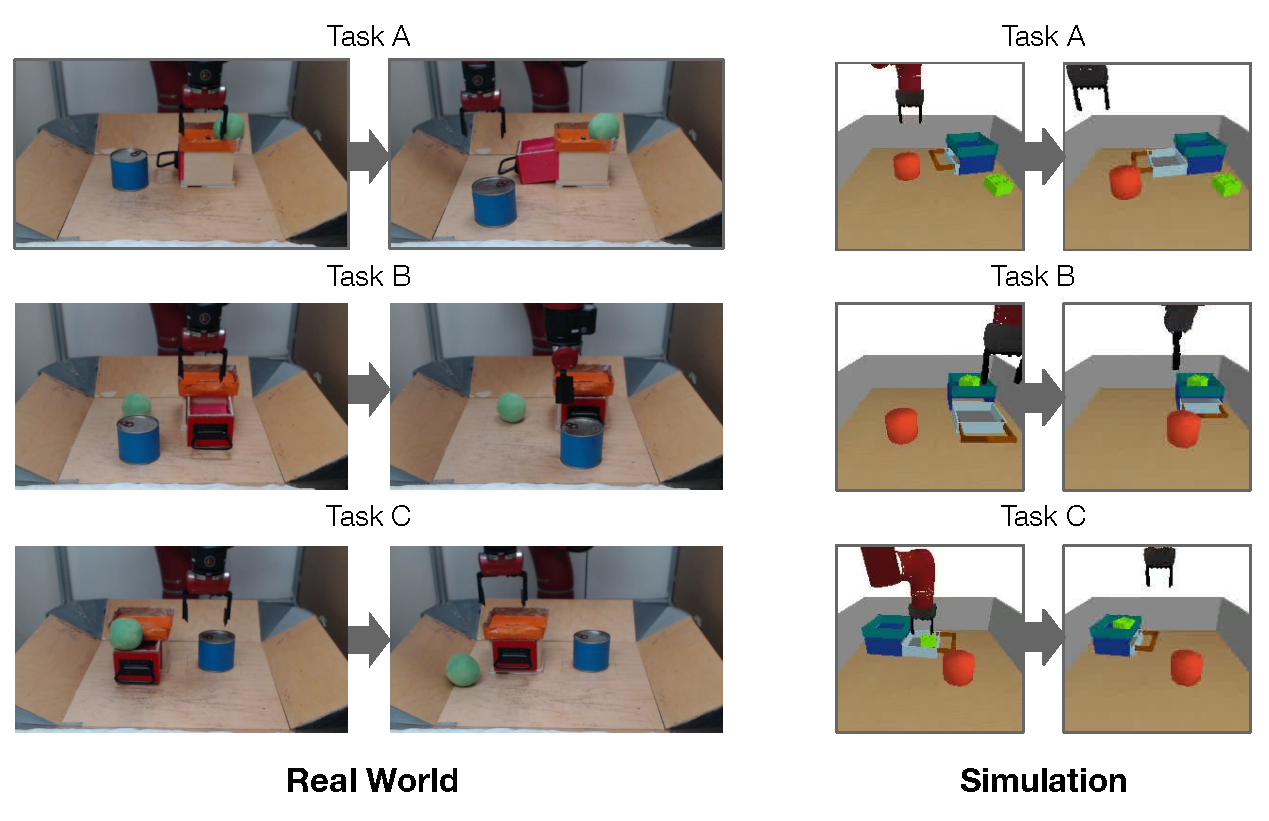
\includegraphics[width=.8\textwidth]{ptp/figures/target_tasks.pdf}
    \vspace{-3mm}
    \caption{\textbf{Target tasks.} Three multi-stage tasks are designed for our experiments in the simulation and the real world respectively. In each target task, the robot needs to strategically interacts with the environment (\eg first takes out an object in the drawer then closes the drawer). The initial state and the desired goal state are shown for each task. }
    \vspace{-5mm}
    \label{fig:target_tasks}
\end{figure}

\vspace*{.3cm}
\begin{figure*}[ht!]
    \centering
    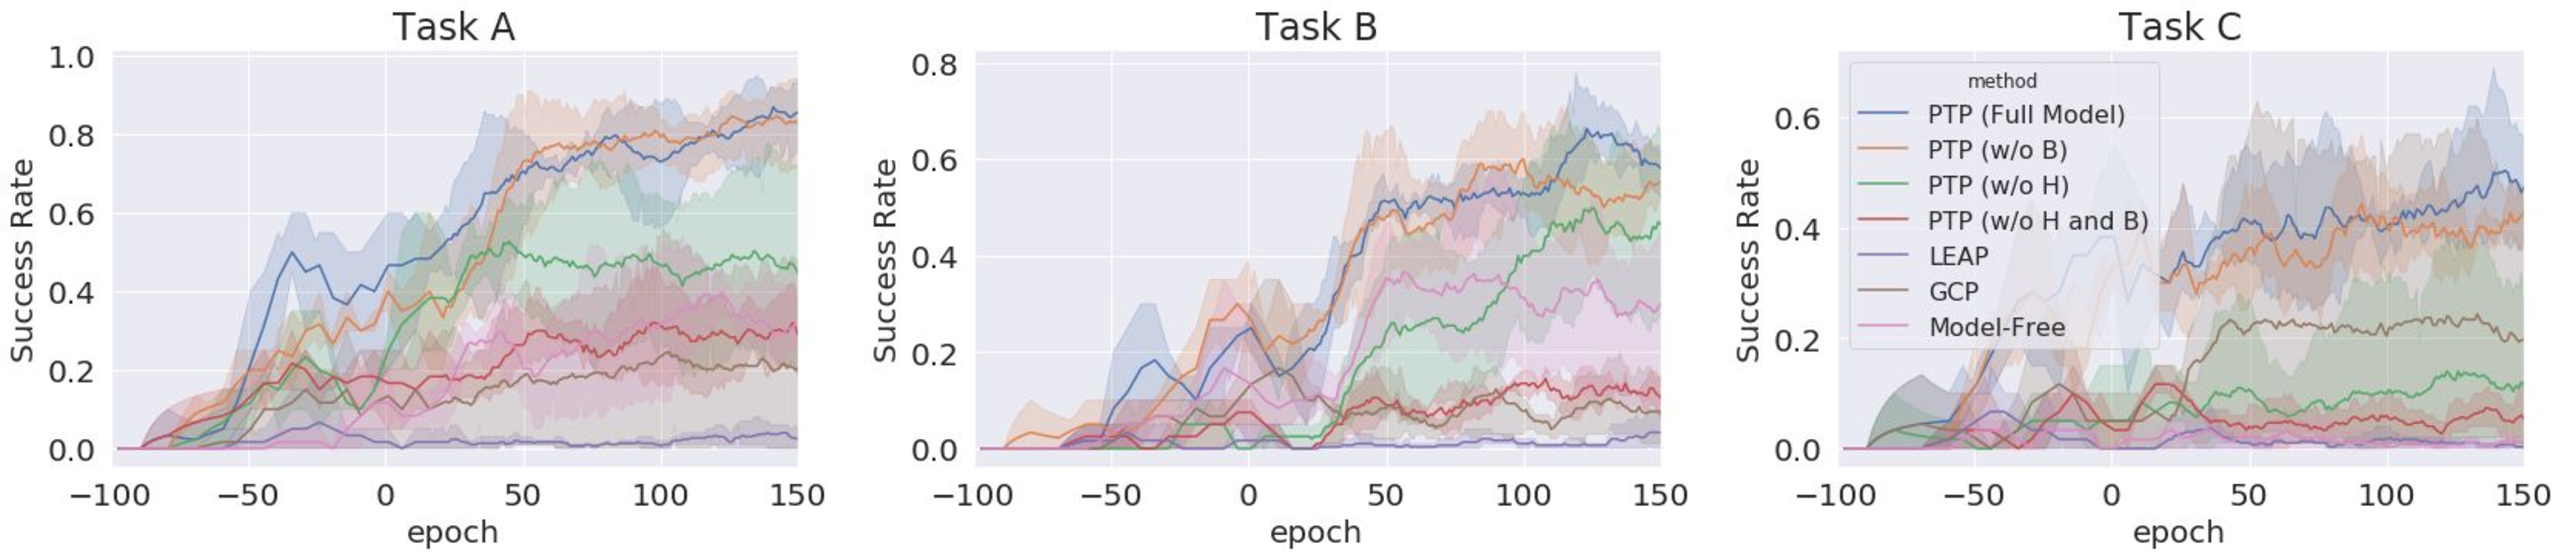
\includegraphics[width=0.95\textwidth]{ptp/figures/sim_quantitative.pdf}
    \vspace{-3mm}
    \caption{
    \textbf{Quantitative comparison in simulation.} The average success rate across 3 runs is shown with the shaded region indicating the standard deviation. The negative x-axis indicates the epochs of offline pre-training and positive x-axis indicates epochs of online fine-tuning.  
    % This figure will show the success rates of all methods (including the baselines and ablations) for the three target tasks.
    Using offline learning and planning, our method PTP is able to solve these tasks partially (at 0 epochs).
    Then with online finetuning the performance improves further.
    In contrast, prior methods have lower offline performance and do not fine-tune successfully in most cases, as they do not collect coherent online data.
    }
    \vspace{-5mm}
    \label{fig:sim_quantitative}
\end{figure*}

% ----------------------------------------------------------------------------------------
\subsection{Cost Function For Feasible Subgoals}

% Planing objective. 
    % - Intuition: Reach the goal & transitions should be probable
    % - Reach the goal
    % - Sampling from the affordance model encourages the transitions to be likely.
% At beginning of each episode, we plan for a sequence of feasible subgoals that leads to the desired goal state of the target task from the initial state. The subgoals are chosen through sampling-based planning, in which we first sample $n$ sequences of subgoals $\hat{s}_{0:k}$ using the conditional goal generator and then evaluate the cost $c(\hat{s}_{0:k})$ of each sequence. 

To provide informative guidance to the policy $\pi(a | s, s_g)$, we would like that the final goal $s_g$ can be reached at the end of the episode while encouraging the transition between each pair of subgoals to be feasible within a limited time budget. As explained in Sec.~\ref{sec:preliminaries}, the goal state is considered to be reached when the Euclidean distance
%%SL.2.24: The Euclidean distance bit will come across as pretty confusing, given that previously we talked about using images -- so readers will wonder, does this mean that we are doing Euclidean distance over images? But that doesn't really make sense.
%%KF.3.1: Clarified.
between the last subgoal in the plan and the desired goal is less than a threshold $\delta$ in the learned latent space. The feasibility of each transition between adjacent subgoals can be measured using the goal-conditioned value function $V(s, s')$ trained by the reinforcement learning algorithm. Therefore, finding the subgoals $\hat{s}_{1:K}^*$ can be formulated as a constrained optimization problem: 
\begin{eqnarray}\label{eqn:constrained_optimization}
    \text{minimize} 
    & \quad & ||s_g - \hat{s}_K|| \\
    \text{subject to} 
    % & \quad & V(s_0, \hat{s}_1) \geq \delta\\
    & \quad & V(\hat{s}_i, \hat{s}_{i+1}) \geq \delta, \text{for $i = 0, ..., K-1$} \nonumber
\end{eqnarray}
where we use $\hat{s}_0 = s_0$ to denote the initial state for convenience. By re-writing Eq.~\ref{eqn:constrained_optimization} as a Lagrangian,
%%SL.2.24: The previous equation has three terms, but perhaps it can be written more concisely so that there is just one constraint (i.e., the line V(s_0, \hat{s}_1) \geq \delta is omitted), if we are careful with our notation.
%%KF.3.1: Fixed.
we obtain the cost function with a weight $\eta$:
\begin{equation}
    c(s_0, \hat{s}_{1:K}, s_g) = ||s_g - \hat{s}_K|| + \eta \sum_{i=0}^{K-1} V(\hat{s}_i, \hat{s}_{i+1})
    \label{eqn:cost_function}
\end{equation}
% where $\eta$ is a weight that balances the two terms. 
The details of our method are explained in Sec.~\ref{sec:implementation_details}.
\section{Experiments}

In our experiments, we aim to answer the following questions: 1) Can PTP propose and select feasible subgoals as plans for real-world robotic manipulation tasks? 2) Can the subgoals planned by PTP facilitate online fine-tuning of the goal-conditioned policies to solve target tasks unseen in the offline dataset? 3) How does each design option affect the performance of PTP?
% To answer these questions, we conduct experiments in both the simulation and the real world. 
Videos of our experimental results are available on the project website: \href{https://sites.google.com/view/planning-to-practice}{sites.google.com/view/planning-to-practice}

% \begin{enumerate}
%     \item Can PTP achieve strong performance after finetuning on goal-conditioned robotic manipulation tasks?
%     % \item Does PTP outperform prior methods on goal-conditioned simulated tasks? %%AVN.2.27 How should we separate sim vs real
    
%     \item Can PTP produce novel multi-stage strategies by composing the primitive behaviors seen in the prior data in new ways?
%     %%SL.2.24: This is a really important question, but maybe we can make this more explicit (i.e., by composing the primitive behaviors seen in the prior data in new ways)
%     %%PY.2.27: fixed
    
%     %%\item Can PTP generate feasible plans in latent space for solving long-horizon robotic manipulation tasks? %%AVN.2.27 What is the difference between these first two questions?
%     %%PY.2.27 Not much of a difference. Commenting out the second one.

% \end{enumerate}
% %%SL.2.24: maybe the finetuning question should be the first one, so as to avoid creating the impression that the finetuning is an "extra" thing and the method is mostly an imitation learning method -- basically, make it really clear that the online training is essential, and after showing that it works, we'll study all the different cool things that can be done with it (like composing skills in new ways via the planner)
% %%PY.2.27: fixed

% In the following sections, we study these questions in both simulated and real-world robotic manipulation domains. We evaluate and compare PTP with other model-based planning methods model-free RL methods that directly using final goals.
%%SL.2.24: it's not actual clear what its "model-free counterpart" refers to...
%%PY.2.27: fixed

\subsection{Experimental Setup}
\label{sec:experimental_setup}

% We construct a simulated platform to evaluate multi-step manipulation tasks using a real-time physics simulator [16]. As shown in Fig. 1, the workspace setup includes a 7-DoF Sawyer robot arm, a table surface, and a depth sensor (Kinect2) installed overhead. Up to 5 objects are randomly drawn from a subset of the YCB Dataset [17] and placed on the table. The Sawyer robot holds a short stick as the tool to interact with the objects to complete a specified task goal.

\textbf{Environment.}
As shown in Fig.~\ref{fig:target_tasks}, our experiments are conducted in a table-top manipulation environment with a Sawyer robot. At the beginning of each episode, a fixed drawer and two movable objects are randomly placed on the table. The robot can change the state of the environment by opening/closing the drawer, sliding the objects, and picking and placing objects into different destinations, \etc. At each time step, the robot receives a 48 x 48 RGB image via a Logitech C920 camera as the observation and takes a 5-dimensional continuous action to change the gripper status through position control. The action dictates the change of the coordinates along the three axes, the change of the rotation, and the status of the fingers. We use PyBullet~\cite{coumans2021} for our simulated experiments.  

% Our simulated and real-world experiments are identical in setup. The robot has 5 degrees of control: 3 dimensions of end-effector velocity control in Euclidean space, one dimension for rotation along the yaw axis of the end-effector, and one dimension to open and close the end-effector. For our simulation experiments, we use PyBullet \cite{coumans2021}. For our real-world experiments, we use a Sawyer robot.
%%SL.2.24: good place to reference a figure
%%KF.3.1: Fixed.

\textbf{Prior data.}
The prior data consists of varied demonstrations for different primitive tasks. In each demonstrated trajectory, we randomly initialize the environment and perform primitive interactions such as opening the drawer and poking the object. These trajectories are collected using teleoperation in the real world, and a scripted policy that uses privileged information of the environment (e.g., the object pose and the status of the drawer) in simulation. The trajectories vary in length from 5 to 150 time steps, with 2,344 trajectories in the real world and 4,000 in simulation.

% Randomly selected
% %%SL.2.24: you said before it was expert? now it's random?
% %%AVN.2.27 fixed
% rollouts from our prior data in our simulated multi-task environment are shown in Figure \ref{fig:sim_primitive_tasks}. The prior data is used to train the VQ-VAE and CVAE and used for offline RL pretraining. Each trajectory of our prior dataset consists of a noisy expert policy interacting with one of the three objects in our environment: a drawer, a slidable object, and a graspable object. This includes
% %%SL.2.24: this is easy to misunderstand as having a discrete hand-coded set of primitives (whereas in reality we have goals)
% %%PY.2.27: fixed
% \begin{itemize}
%     \item Opening or closing a drawer by the handle
%     \item Sliding a large object to an adjacent quadrant
%     \item Moving a small object via grasping in between inside the drawer, on top of the drawer, and any valid location on the table surface
% \end{itemize}

% One important note is that the notion of skills is not used in our model since our model is only conditioned on the image of the current state and the image of the goal state.
% % One important note is that we define these skills only for the purpose of collecting demonstrations. The notion of skills is not used in our model, and each skill can be broken down into more fine-grained behaviors. At the finest level, our planner aims to compose these primitive behaviors.

% %%SL.2.24: This is an important point, but I wonder if we can just tweak the phrasing in the preceding paragraphs to avoid referring to these as "skills" or "primitives" entirely or, failing that, find some way to clarify this paragraph?
% %%PY.2.27: Fixed. I tweaked the phrasing to avoid referring to these as "skills" or "primitives".

% The noisy expert policy used during data collection is a scripted policy with added Gaussian noise in simulation and a human teleoperator in the real-world. Every $K$ trajectories of data collection, we randomly select a new valid position and orientation for the drawer and objects. Further details about data collection are shown in Appendix \ref{appendix:experimental_details}.
% %%SL.2.24: I think readers will have *a lot* of questions about what this "noisy expert" is. The performance of the method and the difficulty of the tasks is very strongly dependent on understanding what the data is and where it comes from, and the description here is quite terse -- I think we should give more of an explanation, perhaps with some examples
% %%PY.2.27: fixed

\textbf{Target tasks.} 
In each target task, a desired goal state is specified by a 48 x 48 RGB image (same dimension with the observation). The robot is tasked to reach the goal state by interacting with the objects on the table. Task success for our evaluation is determined based on the object positions at the end of each episode (this metric is not used for learning). As shown in Fig.~\ref{fig:target_tasks}, we design three target tasks that require multi-stage interactions with the environment to complete. These target tasks are designed with temporal dependencies between stages (\eg the robot needs to first move away a can that blocks the drawer before opening the drawer). The transitions from the initial state to the goal state are unseen in the offline data. The episode length is 400 steps in simulation and 125 steps in the real world, which are much longer than the time horizon of the demonstrations. 

\textbf{Baselines and ablations.} 
We compare PTP with 3 baselines and 3 ablations. \textbf{Model-Free} uses a policy directly conditioned on the final goal and conducts online fine-tuning without using any subgoals. \textbf{LEAP}~\cite{Nasiriany2019PlanningWG} learns a variational auto-encoder (VAE)~\cite{kingma2014vae} to capture the prior distribution of states and plans for subgoals without conditioning on any context. \textbf{GCP}~\cite{Pertsch2020LongHorizonVP} learns a goal predictor that hierarchically generates intermediate subgoals between the initial state and the goal state. To analyze the design options in PTP, we also compare with variations of our method by removing the latent plan buffer (\textbf{PTP (w/o B)}), the hierarchical planning algorithm (\textbf{PTP (w/o H)}), and both of these two designs (\textbf{PTP (w/o H and B)}). All methods use the same neural network architecture in the goal-conditioned policy and are pre-trained on the same offline dataset.

\subsection{Implementation Details}
\label{sec:implementation_details}
% \kuan{In progress. Moving all implementation details here.}

%%In PTP, we collect an offline dataset $\mathcal{D}$, train representation learning, train offline RL, and finally run online RL for a specific environment. 



Following \cite{Khazatsky2021WhatCI}, we use a vector quantized variational autoencoder (VQ-VAE)~\cite{Oord2017NeuralDR} as the state encoder, which encodes a $48 \times 48 \times 3$ image to a 720-dimensional encoding. The conditional subgoal generator is implemented with a U-Net architecture~\cite{Ronneberger2015UNetCN} and decodes the subgoal from a 8-dimensional latent representations conditioned on the encoding of the current state. In our planner, we use $L = 3$, $K = 8$, $M = 2$, $N = 1024$, and we run MPPI for 5 iteration on each level. $g$ is trained to predict subgoals that are 15, 30, and 60 steps away. Implicit Q-Learning (IQL)~\cite{kostrikov2021iql} is used as the underlying RL algorithm for offline pre-training and online fine-tuning with default hyperparameters. We use the same network architectures for the policy and the value functions from ~\cite{Khazatsky2021WhatCI} for simulation experiments. For real-world experiments, we use a convolutional neural network instead. We use Adam optimizer with a learning rate of $3 \cdot 10^{-4}$ and a batch size of 1024. During training, we relabel the goal with future hindsight experience replay~\cite{Andrychowicz2017HindsightER} with $70\%$ probability. We use $\epsilon=3$ for the reward function defined in Sec.~\ref{sec:preliminaries}, $\eta = 0.01$ in Eqn.~\ref{eqn:cost_function}. 

% We also use a CVAE in $h$-space to generate subgoals. The VQ-VAE and CVAE are pre-trained on the offline dataset and its weights are fixed during online fine-tuning. We run offline RL using IQL ~\cite{kostrikov2021iql} and fine-tune in a specific environment with online RL. Our policy, Q-network, and value network are fully connected networks. Our reward function is $r(h, h_g) = -\mathds{1}_{\|h-h_g\| > \epsilon}$. For any transition $(s_t, a_t, r_t, s_{t+1}, s_g)$ during training, we also sample a new goal $s_g'$ with some probability, recompute $r_t'(s_{t+1}, s_g)$, and use this relabeled transition for off-policy Bellman updates. The relabeled goal $s_g'$ may come from future states in a transition~\cite{Andrychowicz2017HindsightER}, a random sample from the replay buffer~\cite{pong2018tdm}, or a random sample from learned goal distribution~\cite{nair2018rig}. 

% During training, we relabel the goal with future hindsight experience replay with $60\%$ probability and the next observation with $10\%$ probability. Our RGB images are 3x48x48, which the VQ-VAE encodes into length-720 vectors. We generate 8 subgoals when planning during finetuning, and the last subgoal is replaced by the final goal. For RL training, we use the Adam optimizer, a learning rate of $3 \cdot 10^{-4}$, weight decay of 0, batch size of 1024, reward scaling of 1, quantile of $.9$, $\beta=.01$, and $\epsilon=3$ (for sim) and $\epsilon=2$ (for real). During finetuning, we add a fixed Gaussian noise with standard deviation of $.15$. During evaluation, there is no noise added. We have a separate replay buffer for online data and offline data, and during training, sample $60\%$ from the online replay buffer and $40\%$ from the offline replay buffer. Our policy has 4 intermediate hidden layers of size 256, and our Q and V-networks have 2 intermdiate hidden layers of size 256. For our Q-network, we clamp the output at 0. Additional hyperparameters for training PTP and our code are available on the project website: \href{https://sites.google.com/view/planning-to-practice}{sites.google.com/view/planning-to-practice}.


% Prior work has shown that off-policy relabeling of goals can significantly improve the sample efficiency of goal-conditioned RL algorithms~\cite{Andrychowicz2017HindsightER}.
% %%SL.3.1: probably not the right place for prior work discussion... should keep this brief and factual if possible
% For any transition $(s_t, a_t, r_t, s_{t+1}, s_g)$, one can sample a new goal $s_g'$, recompute $r_t'(s_{t+1}, s_g)$, and use this relabeled transition for off-policy Bellman updates. The relabeled goal $s_g'$ may come from future states in a transition~\cite{Andrychowicz2017HindsightER}, a random sample from the replay buffer~\cite{pong2018tdm}, or a random sample from learned goal distribution~\cite{nair2018rig}.


% During finetuning and evaluation, we provide the robot an image of the goal state. To reach this goal state from its current state, the robot must sequence together multiple atomic behaviors. Importantly, the target tasks are temporally extended. The pair of initial state and the goal state in each target task is unseen during pretraining. The three target tasks are shown in Figure \ref{fig:sim_target_tasks}. Below are some brief descriptions of the three tasks:
% \begin{itemize}
%     \item Task 1. Close the drawer and then push the large object in front of the drawer.
%     \item Task 2. Push the large object out of the way and then open the drawer
%     \item Task 3. Take the small object out of the drawer, put it on top of the drawer, and then close the drawer.
% \end{itemize}

% Note that the atomic behaviors required to accomplish the target task are also temporally dependent. For instance, in task 1, the robot cannot push the large object in front of the drawer if it does not first close the drawer because the drawer is blocking the large objects' path. 
% We created three target tasks to fine-tune and evaluate over in both our simulation and real-world environment. 
% Specifically, we first arrange objects in the environment into an initial state. Then, we provide a goal image of objects in the environment arranged differently, so that the robot must accomplish a long-horizon task in order to reach a scene that resembles the goal image. Here, a long-horizon task consists of two temporally dependent primitive skills accomplished in sequence. 

%%SL.2.24: This is all rather vague, perhaps provide examples of start and goal states and explain how they require sequencing multiple atomic behaviors to reach the goals successfully
%%PY.2.27: fixed

%%KF.2.28: We should probably remove this figure. We can still put it on our website.
% \begin{figure}[t!]
%     \centering
%     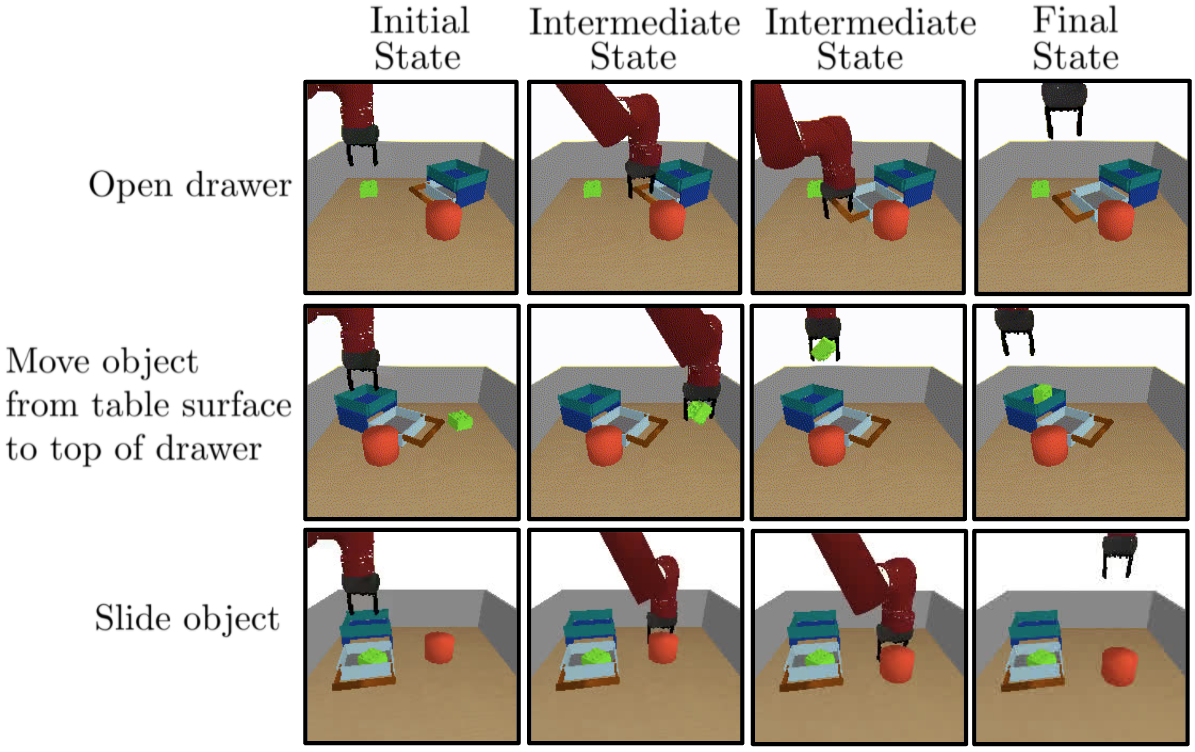
\includegraphics[width=.45\textwidth]{figures/sim_primitive_tasks.png}
%     \caption{Prior data. Each row contains one randomly sampled trajectory from the prior data, which involves the scripted policy accomplishing a primitive skill.}
%     \label{fig:sim_primitive_tasks}
% \end{figure}


% \begin{figure}[t!]
%     \centering
%     \includegraphics[width=.4\textwidth]{example-image-a}
%     \caption{Real-World Tasks. This figure shows the initial and goal states in each target task in real world.}
%     \label{fig:real_target_tasks}
% \end{figure}


% \subsection{Fine-Tuning on Long-Horizon Tasks} 
% %%SL.2.24: the "non-episodic" bit is mentioned for the first time here, hard to understand
% %%AVN.2.27 changing the section title

% We evaluate our method and baselines on our three target tasks in both our simulation and real-world environment. The baselines we evaluate include

% \textbf{Model-Free (VAL)~\cite{Khazatsky2021WhatCI}} This method does not use planning with subgoals during exploration. Instead, the policy is conditioned on only the final goal.

% \textbf{GCP~\cite{Pertsch2020LongHorizonVP}} This method learns a goal-conditioned predictor which predicts an intermediate subgoal between the initial state and goal state that is fed into it. The predictor is trained hierarchically by recursively subdividing each part of the trajectory. The hierarchical planner used during exploration utilizes this predictor to optimize trajectories in a coarse-to-fine manner.

% \textbf{LEAP~\cite{Nasiriany2019PlanningWG}} This method learns a variational auto-encoder (VAE)~\cite{kingma2014vae} and plans over latent variables in the VAE latent space. LEAP used a temporal difference model (TDM)~\cite{pong2018tdm} to determine the reachability of latent subgoals. As there is no implementation of TDM that utilizes offline data, we instead use the same value function as our method to determine reachability, also making the two methods more comparable.

% % \textbf{SORB \cite{Eysenbach2019SearchOT}} This method samples one intermediate subgoal from the replay buffer during planning rather than from an affordance model.



\begin{figure}[t!]
    \centering
    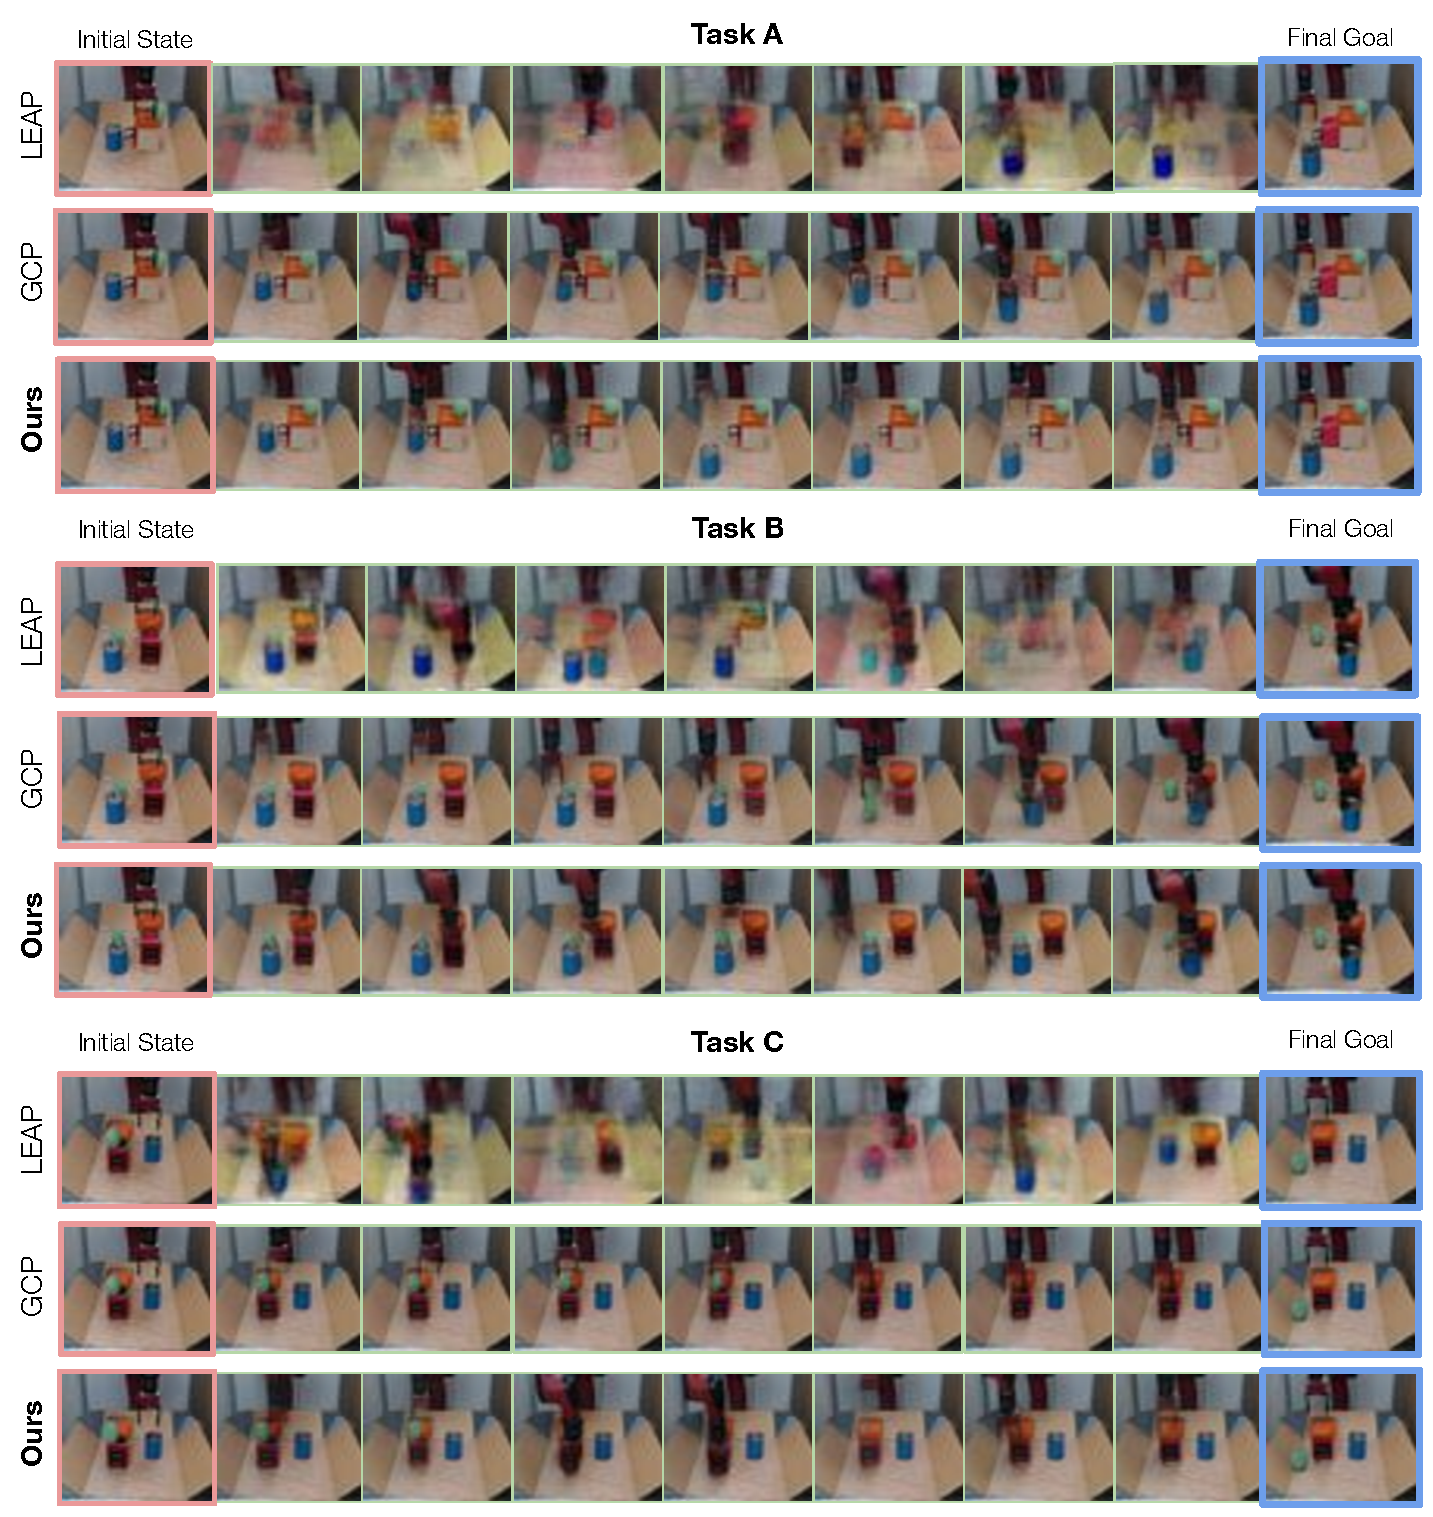
\includegraphics[width=.8\textwidth]{ptp/figures/real_qualitative.pdf}
    % \vspace{-3mm}
    \caption{\textbf{Planned subgoal sequences.} Each row shows the sequence of subgoals produced by each method. The initial state and the final goal are shown at the two ends. 
    % Due to optimizing over an unconditional latent variable, subgoals from LEAP are incoherent. The sequence of images from GCP between the initial and goal image is smooth, but do not actually contain dynamically reachable subgoals. The planned subgoal sequence from our method in contrast successfully interpolates between the initial state and goal state to provide meaningful subgoals to the lower-level goal-conditioned policy.
    %%SL.3.1: same comment, please add a real caption
    }
    \vspace{-5mm}
    \label{fig:real_qualitative}
\end{figure}

\subsection{Quantitative Comparisons}

We evaluate PTP and baselines on three unseen target tasks. We use simulated versions of these tasks for comparisons and ablations, and real-world tasks, where all pretraining and finetuning uses only real-world data, to evaluate the practical effectiveness of the method.

\textbf{Simulation}. We first pre-train the goal-conditioned policy on the offline dataset for 100 epochs and the run online fine-tuning for the target task for 150 epochs. Each epoch takes 2,000 simulation steps (only during fine-tuning) and 2,000 training iterations. We run online fine-tuning using each method with 3 different random seeds. After each epoch, we test the policy in the target task for 5 episodes. We report the average success rate across 3 runs in Fig.~\ref{fig:sim_quantitative} where the negative x-axis indicates the offline pre-training epochs and positive x-axis indicates the online fine-tuning epochs.

As shown in Fig.~\ref{fig:sim_quantitative}, our full model consistently outperforms baselines with a large performance gap. The generated subgoals not only enables the pre-trained policy to achieve higher success rate by breaking down the hard problems into easier pieces, but also introduces larger performance improvements during online fine-tuning. After fine-tuning for 150 epochs, the policy achieves the success rates of 84.9\%, 59.9\%, 49.3\% in the three target tasks respectively. Compared to the policy pre-trained on the offline dataset, the performance is significantly improved (+31.6\%, +37.8\%, and +13.8\%). When directly using the final goal or subgoals generated by baseline methods, the policy's performance plateaus at around 0.0\% to 30.0\% and does not improve much during online fine-tuning. 

We found that the hierarchical planner and the latent plan buffer are crucial for PTP's performance. Without these two design options, the planner often suffers from the large search space of possible subgoal sequences and the resultant success rates decrease. The latent plan buffer significantly improves the performance of non-hierarchical PTP while it has a minor effect on hierarchical PTP.   

\textbf{Real-world evaluation.} We pre-train the policy for 200 epochs and fine-tune it for 10 epochs. In each epoch, we run 10,000 training iterations and collect 1,000 steps in the real world. We train on three target tasks which are shown in Figure~\ref{fig:target_tasks}, and report the success rate of the goal-conditioned policy before and after online fine-tuning in Table~\ref{fig:real_quantitative}. Planning enables the robot to succeed partially with just the offline initialized policy, achieving success rates of $12.5\%, 75.0\%$ and $25.0\%$ on the three tasks. (When the offline policy is conditioned on only the final goal image without planning, the success rate is $0\%$.) Then in each task, we fine-tune to a significantly higher success rate.

Qualitatively, at the beginning of fine-tuning, the robot often fails, deviating from the planned subgoals or colliding with the environment.
With the planned subgoals, the original long-horizon task is broken down to short snippets that are easier to complete.
Even if a subgoal is not reached successfully at first, the data is useful to collect additional experience and fine-tune the policy.
After fine-tuning for 4-5 epochs, we already observe that the robot's performance reaching subgoals during training time significantly improves, collecting even more coherent and useful data.
After 10 epochs, we achieve success rates of $62.5\%, 100.0\%$ and $50.0\%$.
In comparison, GCP cannot provide useful guidance to the policy when the generated goals are noisy.
%%SL.3.1: Given that this is our main result, it would be good to have a bit more in-depth discussion of what the results actually are, and maybe point to some qualitative results in a figure somewhere.


% \begin{figure}[t!]
% \captionof{table}{The real-world success rates before and after online fine-tuning. The tasks are described in Sec.~\ref{sec:experimental_setup}.}
\begin{table}[t!]
    \normalsize
    \centering
    \caption{The real-world success rates before and after online fine-tuning. The tasks are described in Sec.~\ref{sec:experimental_setup}.}
    \begin{tabular}{ c|c|c }
        \centering
        Task & \begin{tabular}{@{}c@{}}PTP (Ours) \\ Offline $\rightarrow$ \text{Online} \end{tabular} & \begin{tabular}{@{}c@{}} GCP \\ Offline $\rightarrow$ \text{Online} \end{tabular} \\
        \hline
        % (1) Close drawer, slide can & $25.0\% \rightarrow \textbf{62.5\%}$ & $0.0\% \rightarrow 0.0\%$ \\
        % (2) Slide can, open drawer & $12.5\% \rightarrow \textbf{62.5\%}$ & $0.0\% \rightarrow 0.0\%$ \\
        % (3) Poke object, close drawer & $12.5\% \rightarrow \textbf{100\%}$ & $12.5\% \rightarrow 37.5\%$ \\
        % Task A & $25.0\% \rightarrow \textbf{62.5\%}$ & $0.0\% \rightarrow 0.0\%$ \\
        % Task B & $12.5\% \rightarrow \textbf{62.5\%}$ & $0.0\% \rightarrow 0.0\%$ \\
        % Task C & $12.5\% \rightarrow \textbf{100\%}$ & $12.5\% \rightarrow 37.5\%$ \\
        Task A & $12.5\% \rightarrow \textbf{62.5\%}$ & $12.5\% \rightarrow 0.0\%$ \\
        Task B & $75.0\% \rightarrow \textbf{100.0\%}$ & $50.0\% \rightarrow 75.0\%$ \\
        Task C & $25.0\% \rightarrow \textbf{50.0\%}$ & $25.0\% \rightarrow 12.5\%$ \\
    \end{tabular}
    \label{fig:real_quantitative}
    \vspace{-6mm}
\end{table}
% \end{figure}

\subsection{Generated Subgoals}

In Fig.~\ref{fig:real_qualitative}, we present qualitative results of the generated subgoals for each task in the real world. Each row shows a sequence of generated subgoals produced by the planner in each method. In all the three target tasks, PTP successfully plans for a sequence of subgoals that can lead to the desired final goal. The transition between adjacent subgoals are feasible within a short period of time. By comparison, both of the baseline methods fail to generate reasonable plans. Without conditioning on the current state, LEAP~\cite{Nasiriany2019PlanningWG} can hardly produce any realistic images of the environment. Most of the generated subgoals are highly noisy images with duplicated robot arms and objects. The quality of the subgoals produced by GCP~\cite{Pertsch2020LongHorizonVP} is higher than that of LEAP but still much worse than ours. GCP cannot generalize well for the initial state and the goal state that are out of the distribution of the offline dataset, which contains only short snippets of demonstrations.
\section{Conclusion and Discussion}

We presented PTP, a method for real-world learning of temporally extended skills by utilizing planning and fine-tuning to stitch together skills from prior data.
First, planning is used to convert a long-horizon task into achievable subgoals for a lower level goal-conditioned policy trained from prior data.
Then, the goal-conditioned policy is further fine-tuned with active online interaction, mitigating the distribution shift between the offline data and actual states seen during rollouts.
This procedure allows robots to extend their capabilities autonomously, composing previously seen data into more complicated and useful skills.

\section{Contribution Statement}

The work in this chapter was performed in collaboration with Kuan Fang, Patrick Yin, and Sergey Levine~\citep{fang2022ptp}. K.F. and P.Y. were joint first-coauthors. The idea of using an affordance model to set goals for finetuning was developed jointly by K.F. and A.N. The project was primarly managed by K.F. The majority of the simluation experiments were conducted by K.F. and P.Y. The first three authors conducted baseline experiments. The real-world experiments were conducted primarily by P.Y. with assistance from K.F. and A.N. The paper was written by K.F., with A.N. assisting. S.L. advised the project and assisted with writing.

% \newpage

% {\small
% \bibliographystyle{bibtex/IEEEtran}
% \bibliography{bibtex/references}
% }

% \newpage
% \clearpage
% % \appendix
% % %% (Patrick) Moved to experiments section
% \subsection{Implementation Details}
% \label{appendix:implementation_details}
% In PTP, we collect an offline dataset $\mathcal{D}$, train representation learning, train offline RL, and finally run online RL for a specific environment. 

% In the representation learning phase, we first train the VQ-VAE on $\mathcal{D}$ ~\cite{Oord2017NeuralDR}. The VQ-VAE encodes our images from our $[0,1]^{64\times 64\times 3}$ observation space into a length-720 latent vector $\mathbb{z}$. We then encode the entire dataset with the VQ-VAE to obtain discrete latent variables, and then train our conditional subgoal generator on the discrete latent code dataset.

% In the offline RL phase, we run IQL ~\cite{kostrikov2021iql} on the discrete latent code dataset to obtain a single policy and Q-function. This policy and Q-function can then be fine-tuned to a specific environment by running online RL. During training, we relabel the goal with future hindsight experience replay with $60\%$ probability and the next observation with $10\%$ probability.

% All hyper-parameters are provides below for these algorithms in tables ~\cref{tab:rl_hyperparams}, _, _, _, and _.

% \begin{table*}[]
%     \centering
%     \begin{tabular}{c|c}
%       Hyper-parameter  & Value \\
%       \hline
%       $\gamma$  &  $.99$ \\
%       Batch Size & 1024 \\
%       Policy Learning Rate & $3 \dot 10^{-4}$ \\
%       Policy Weight Decay & $0$ \\
%       Q-Network Learning Rate & $3 \dot 10^{-4}$ \\
%       Q-Network Weight Decay & $0$ \\
%       $\beta$ & 0.01 \\
%       $\epsilon$ & 3.0 \\
%     \end{tabular}
%     \caption{Hyper-parameters}
%     \label{tab:hyperparams}
% \end{table*}


% We use a VQ-VAE to encode our images from 3x48x48 to length 720. We modify a PyTorch implementation of  for our offline RL algorithm. Our policy is fully connected network consisting of 4 intermediate layers of size 256. Our Q-network and value network are fully connected networks consisting of 2 intermediate layers of size 256. 


% The hyperparameters used for the experiment are in ~\cref{tab:hyperparams}. We use two replay buffers, one storing online trajectories and one storing offline trajectories, and sample proportionally from the two at training time. 

% \begin{table*}[]
%     \centering
%     \begin{tabular}{c|c}
%       Hyperparameter  & Value \\
%       \hline
%       $\gamma$  &  $.99$ \\
%       Batch Size & 1024 \\
%       Policy Learning Rate & $3 \dot 10^{-4}$ \\
%       Policy Weight Decay & $0$ \\
%       Q-Network Learning Rate & $3 \dot 10^{-4}$ \\
%       Q-Network Weight Decay & $0$ \\
%       $\beta$ & 0.01 \\
%       $\epsilon$ & 3.0 \\
%     \end{tabular}
%     \caption{Hyperparameters}
%     \label{tab:hyperparams}
% \end{table*}




\subsection{Simulation Experimental Details}
\label{appendix:simulation_experimental_details}
Our simulated dataset consists of 4,000 trajectories (300,000 transitions). Every 4 trajectories, we randomize the position and orientation of the drawer, slidable object, and graspable object in the following ways. The position of the drawer is randomly selected between the back two quadrants. The orientation of the drawer is randomly selected such that it doesn't collide into the surrounding wall. The position of the slidable object is randomly selected between the four quadrants such that it doesn't collide with the drawer. The position of the graspable object is randomly selected between inside the drawer, on top of the drawer, or on top of the table. If the graspable object is on top of the table, its position on top of the table is randomly selected such that it doesn't collide with the drawer or slidable object. The yaw of the graspable object is randomized. 

% The trajectories are generated by a scripted policy with added Gaussian noise of .05. which collects play data by interacting with all the present
% objects in a random order.\textcolor{red}{TODO(Patrick)}

% % \textbf{Real-world setting.} Randomly selected workspaces in our real-world environment is shown in \textcolor{red}{TODO(Patrick): Add figure}. Here, a Sawyer robot is controlled at \textcolor{red}{TODO(Patrick): ?}Hz. Our real-world setting mirrors our simulated setting in that both share the same robotic manipulation tasks, sampling scheme for generating a new environment, and degrees of control of the robot.

% % Our real-world dataset consists of \textcolor{red}{TODO(Patrick): ?} trajectories (x transitions) collected by using a 3Dconnexion SpaceMouse device. Instructions for interfacing with the SpaceMouse is available publicly on  \href{https://github.com/vitchyr/rlkit/tree/master/rlkit/demos/spacemouse}{Github}, with the
% % device code adapted from the RoboSuite library \cite{zhu2020robosuite}. \textcolor{red}{TODO(Patrick): More description here once we figure out the real world stuff



% \textcolor{red}{Patrick (Real World Details)}: The three target tasks are:
% \begin{enumerate}
%     \item Close the drawer and push can in front of drawer
%     \item Push can out of drawer's way and open drawer
%     \item Poke object out to the right of the drawer and close drawer
% \end{enumerate}

% For Task 1, we consider a rollout a success if the robot closes the fully-opened drawer more than halfway and pushes the can in front of the drawer. The pretrained policy has some success with closing the drawer from the initial position (37.5\%). The failure case arises with the transition between closing the drawer and pushing the can. The gripper must both rotate 90 degrees and go behind the can in order to push it in front of the drawer. The pretrained policy often struggles with this as it is easy to land upon unseen states during this transition. For instance, the gripper moves too far back in the scene during the transition and cannot recover by moving forward towards the can. Instead it gets stuck and performs seemingly random actions in that area. After finetuning, success rate of drawer opening increases (75\%). More importantly, the policy has an increased success in transitioning between closing the drawer and pushing the object. 

% Interestingly, the pretrained policy also has many different strategies initially on how to transition due to the diversity in the prior data. Sometimes, it tries to go over and behind the can. Other times, it tries to go around and behind the can. After finetuning, it converges upon the strategy of going around and behind the can, likely since there was more success doing this in the earlier epochs of finetuning. Also, the gripper learns a novel strategy to hit singularity in order to push the drawer by over rotating past its physical limits. \textcolor{red}{(Maybe best not to include this actually)} Note that in the prior data, the robot never hits singularity.

% For Task 2, we consider a rollout a success if the robot pushes the can out of the drawer's way and opens the drawer at least halfway. The pretrained policy has great success with sliding the can (87.5\% success), but it again struggles to transition to opening the drawer after doing the can sliding. When the the gripper starts moving back to the handle after sliding the can, it often goes too far in and collides with the side of the drawer. If this unseen state is reached, the robot does not recover and gets stuck pushing the side of the drawer. Rarely, the robot is able to lucky not go too far back during the transition and reach the handle. If the robot can make it to this state of being close to the handle, it can very consistently open the drawer. After finetuning, the robot has greater success in not going too far back during the transition and getting stuck. Note that to get this working, we had to constrain the rotation of the gripper within $\pi / 2$ to prevent it from hitting singularity. Also we had to constrain the z-dimension so that the robot cannot move past the top of the drawer. If we don't set these constraints, the robot often ends up drifting up too high (where these states are unseen) and cannot recover, instead just wandering around aimlessly.

% For Task 3, we consider a rollout a success if the robot can poke the object to the side of the drawer and close the drawer fully. Note that if the robot pokes the object to different location like the front of the drawer, we consider this to be a failure. The majority of the time, the pretrained policy either fails to close the drawer (37.5\%) or can close the drawer but ignores the object in doing so (50\%). As a result, the object either gets stuck between the gripper and drawer or the object accidently falls onto the table, but often not in the desired location. For instance, it often rolls to the front of the scene. After finetuning, the policy can consistently move rightward explicitly first to push the object on top the table to the right of the drawer, and then close the drawer. Note that we had to constrain the rotation of the gripper within $\pi / 2$ to prevent it from hitting singularity for this task as well.

% When conditioned on only the final goal image after finetuning, the robot goes through the correct high-level motions of the two skills and the transition between them. However, it does this very unprecisely and never succeeds on each skill or the transition between the two skills.

% With GCP, on Task 1 and 2, GCP is never able to succeed. It is able to slide the can, but it fails at opening/closing the drawer. Finetuning doesn't seem to consistently improve the performance of sliding the can, likely since performance is bottlenecked by the noisiness of the subgoals. For Task 3 with GCP, the policy is able to close the drawer the vast majority of the time. However, it runs into the same issue after pretraining where it ignores the object. After finetuning, the policy does a little better at this, although it still ignores the object most of the time (62.5\%). GCP likely works for this task since it is a shorter-horizon task with an easier transition between the two primitive skills. As a result, the model is able to lean more on the goal-conditioned policy and less on the planned subgoals to solve the task.

% \end{document}
